\documentclass[10pt]{article}

\usepackage[margin=1in]{geometry}
\usepackage[T1]{fontenc}
\usepackage[utf8]{inputenc}
\usepackage{amsmath,amssymb}
\usepackage{booktabs}
\usepackage{tabularx}
\usepackage{array}
\usepackage{graphicx}
\usepackage{float}
\usepackage{algorithm}
\usepackage{algpseudocode}
\usepackage{tikz}
\usepackage{xcolor}
\usepackage{hyperref}
\usepackage{microtype}

\usetikzlibrary{arrows.meta,positioning,calc,fit,backgrounds,shapes.geometric}

\graphicspath{{../lie_group_integrator_work/paper_v047_cylindrical_chain/figures/}}

\definecolor{uwred}{HTML}{C00000}
\definecolor{muted}{HTML}{555555}
\definecolor{lightbg}{HTML}{F4F5F7}
\definecolor{paperblue}{HTML}{1F5F99}
\definecolor{papergreen}{HTML}{237A57}
\definecolor{paperorange}{HTML}{B65A12}
\definecolor{papergray}{HTML}{E7E9ED}
\definecolor{paperred}{HTML}{B3261E}

\tikzset{
  paperbox/.style={
    draw=paperblue!70,
    fill=paperblue!7,
    rounded corners=2pt,
    align=center,
    inner sep=4pt,
    minimum height=8mm,
    font=\small
  },
  verifierbox/.style={
    draw=papergreen!75,
    fill=papergreen!8,
    rounded corners=2pt,
    align=center,
    inner sep=4pt,
    minimum height=8mm,
    font=\small
  },
  warningbox/.style={
    draw=paperorange!85,
    fill=paperorange!8,
    rounded corners=2pt,
    align=center,
    inner sep=4pt,
    minimum height=8mm,
    font=\small
  },
  boundarybox/.style={
    draw=paperred!80,
    fill=paperred!7,
    rounded corners=2pt,
    align=center,
    inner sep=4pt,
    minimum height=8mm,
    font=\small
  },
  paperarrow/.style={-{Latex[length=2.2mm]}, thick, draw=muted},
  claimarrow/.style={-{Latex[length=2.2mm]}, thick, draw=paperred!75},
  lane/.style={draw=muted!60, fill=papergray!50, rounded corners=2pt, inner sep=5pt}
}

\newcolumntype{Y}{>{\raggedright\arraybackslash}X}
\newcommand{\method}{Gauss6/FullVA}
\newcommand{\agent}{auto-research agent}
\newcommand{\todo}[1]{\textcolor{uwred}{[TODO: #1]}}

\title{\vspace{-1.0em}
Verifier-Centered Auto-Research Agents for Lie-Group Multibody Integrator Development:\\
A Versioned Case Study}
\author{Jingquan Wang\\Simulation-Based Engineering Laboratory\\University of Wisconsin--Madison}
\date{June 9, 2026}

\begin{document}
\maketitle

\begin{abstract}
Large-language-model agents can edit code, launch experiments, and summarize
logs, but those capabilities are not sufficient for numerical-method research.
In Lie-group multibody dynamics, a candidate integrator can produce an
attractive convergence plot while failing to preserve velocity-level
constraints, relying on an unreported endpoint projection, comparing against an
unfair reference policy, or exceeding what its proof actually establishes.
This paper proposes a verifier-centered architecture for building
domain-specific auto-research agents for constrained Lie-group integrator
development. The central design principle is that the agent must co-design
four objects: the method specification, the verifier sandbox, the proof ledger,
and the numerical example ladder. The resulting workflow represents each
candidate method as an explicit one-step-map object, runs bounded validators
before full artifact generators, separates theorem inputs from diagnostic
evidence, and records claim states as accepted, diagnostic, open, or
forbidden. We ground the architecture in a versioned research tree that evolved
from v001 to v048 for lower-pair multibody integrator work. The current case
study centers on a \method{} path with a conditional sixth-order method claim,
smooth observed position/velocity orders of approximately 7.161/7.066, four
ASME mechanism examples in the evidence system, and explicit nonpromotion
boundaries for full source-paper temporal finite-element replacement,
source-policy external superiority, sparse runtime superiority, and
sharp-friction coarse-regime behavior. The contribution is not a generic
``research agent'' recipe. It is a concrete methodology for using agents in a
research domain where proof obligations, numerical examples, and paper claims
must remain synchronized over many iterations and many contributors.
\end{abstract}

\noindent\textbf{Keywords:} auto-research agents; multibody dynamics;
Lie-group integration; constrained differential-algebraic equations; numerical
verification; proof ledgers; reproducibility.

\section{Introduction}

Multibody simulation is useful only when the time integrator respects the
geometric and algebraic structure of the mechanism being simulated. In rigid
and flexible multibody systems, finite rotations must remain on the relevant
Lie group, bilateral joints must satisfy position-, velocity-, and
acceleration-level constraints, and reaction forces or friction laws may change
the engineering conclusion drawn from the simulation. These requirements make
integrator research different from ordinary software development. A script can
run successfully, a plot can look plausible, and a regression test can pass,
while the method is still not a defensible integrator.

This distinction matters for laboratories that develop simulation methods over
many projects. In one part of the lab, researchers may work on Lie-group
Runge--Kutta or collocation schemes. In another, they may work on lower-pair
constraints, friction/contact laws, sparse Newton solvers, public benchmark
mechanisms, or reproducible paper packages. These activities interact through a
shared evidence space. A change in the stage residual can invalidate a proof
ledger; a change in the reference policy can invalidate a work-precision
comparison; a mechanism that closes position constraints may still be only a
coverage row rather than an accepted asymptotic dynamic-order row. An
\agent{} for this setting is valuable only if it coordinates these dependencies
instead of merely generating code.

This is also why the problem is practically important inside a lab rather than
only philosophically interesting. Multiple researchers may be attacking the
same integrator family from different directions: one person improving a
Gauss-collocation residual, another building an ASME mechanism mapping, another
checking public-code baselines, and another preparing a manuscript. Without a
shared verifier and memory system, those threads can drift into mutually
inconsistent claims. The agent proposed here is a coordination mechanism for
that research ecology: it keeps each person's artifact useful to the others by
recording exactly what the artifact proves, what it only diagnoses, and what it
does not yet justify.

The motivating case in this paper is a versioned research pipeline for
Lie-group, lower-pair multibody integrator development. The pipeline currently
contains a \method{} path, a temporal finite-element (TFE) comparison target,
ASME-style mechanism examples, proof and claim ledgers, and a cross-paper
same-test benchmark scaffold. The artifact state is deliberately bounded. The
accepted local method claim is a conditional sixth-order \method{} claim with
smooth observed position/velocity orders about 7.161/7.066. Four ASME examples
enter the method evidence system; single- and double-pendulum rows support
dynamic-order evidence, while four-link and slider-crank rows support
mechanism coverage and closed-loop consistency unless a stronger
residual-to-error theorem or true dynamic-order campaign is closed. The
pipeline does not claim complete source-paper TFE residual reproduction, full
source-policy external superiority, or sparse runtime superiority.

This paper asks: how should an auto-research agent be built for this kind of
integrator research? The answer proposed here is verifier-centered. The agent
does not treat experiments as a flat task list. It maintains an explicit
method object, chooses a sandbox level before execution, keeps proof
obligations in a separate ledger, selects numerical examples to expose
specific failure modes, and writes paper claims only through a claim-state
machine. In this architecture, autonomy is not measured by how many commands
the agent can run without a human. It is measured by how reliably the agent
prevents unverified claims from crossing the boundary into the paper.

The paper makes four contributions:
\begin{enumerate}
  \item It formulates a domain-specific architecture for auto-research agents
  in Lie-group multibody integrator development.
  \item It defines the core research objects--MethodSpec, ProblemSpec,
  EvidenceSpec, and ClaimSpec--that let an agent preserve method identity and
  paper-claim boundaries.
  \item It introduces verifier and proof sandbox patterns that separate
  read-only validators, bounded audits, full artifact generation, and
  external source-policy campaigns.
  \item It grounds the framework in a v001--v048 versioned case study,
  showing how each phase of the project added a verifier because a previous
  phase exposed a new failure mode.
\end{enumerate}

\section{Background and Motivation}

\subsection{Constrained multibody integration}

Constrained multibody dynamics is commonly formulated as a differential-
algebraic system with kinematic constraints, velocity constraints, acceleration
constraints, and Lagrange multipliers. Classical references on stiff ordinary
differential equations and DAEs emphasize that the numerical method must be
matched to the index and stability structure of the problem
\cite{hairer1996solving,gear1985automatic}. For mechanical systems, the
problem is compounded by rotations. Lie-group integration methods address the
fact that rigid-body orientations are not Euclidean vectors
\cite{munthe1998lie,munthe1999high}. Constrained Lie-group time integration
has therefore become a recurring theme in multibody dynamics
\cite{bruls2012lie,wieloch2021bdf}.

The practical difficulty is that no single plot captures all relevant
properties. Position error, velocity error, constraint drift, multiplier
consistency, Newton convergence, runtime, and reference-policy fairness are
different pieces of evidence. A method that performs well in a smooth
single-body test may fail in a lower-pair mechanism. A method that satisfies
endpoint position constraints may still hide a velocity inconsistency. A method
that has an exact sparse pattern may still lose to a dense automatic
differentiation backend in wall-clock time.

\subsection{Temporal finite elements and comparison targets}

Time finite element methods provide another way to construct high-order
time-integration schemes for structural and multibody dynamics
\cite{borri1988rigid,hughes1988spacetime,hulbert1992time,jog2016robust,bauchau2024time}.
The motivating source-paper family includes higher-order integration of
index-3 DAEs with friction using time finite elements on Lie groups
\cite{chaturvedi2026tfe}. In the local pipeline, the source-paper TFE
formulation and the implemented \method{} path are deliberately distinguished.
The accepted local method claim is not that the complete source-paper residual
has been reimplemented. Rather, the local TFE target appears as a formal-order
comparison object: a paper-style $m=3$ Gauss--Lobatto TFE target with expected
order five, contrasted against the conditional sixth-order \method{} path.

This distinction is a representative example of why an agent needs a claim
ledger. A generic agent may see TFE-related diagnostics, convergence plots, and
source-policy files and compress them into a single statement that ``the TFE
method was reproduced.'' That statement would be wrong. The artifact boundary
is narrower: some formula mappings and diagnostics exist, but
\texttt{full\_tfe\_stage\_replacement=false} remains an open stronger
reproduction target.

\subsection{External baselines and source-policy fairness}

External comparison introduces a second class of failure. A local method may
look superior if it uses a different time window, a different reference
solution, a different error metric, or a different work metric. The relevant
baseline family in the case study includes SBEL/Negrut mechanisms and
rotation-representation work, including exponential-map, absolute-coordinate,
half-implicit, and velocity-partitioning/Lie-group baselines
\cite{taves2020exponential,kissel2021dwelling,kissel2022absolute,fang2023halfimplicit,kissel2024velocitypartitioning}.
The v048 scaffold therefore treats external comparison as a source-policy
object. Until same-test campaigns are run with matched parameters, drivers,
reference policies, error metrics, and work metrics, the claim
\texttt{external\_superiority\_claim=false} remains active.

\section{Problem Statement and Design Requirements}

The task is to build an agent that helps researchers search the space of
integrators, repairs, examples, proofs, and paper claims without corrupting the
evidence boundary. We model the agent as a controller over a research state
\[
  \mathcal{S} = (\mathcal{M},\mathcal{P},\mathcal{E},\mathcal{C},\mathcal{L}),
\]
where $\mathcal{M}$ is the method specification, $\mathcal{P}$ is the problem
or benchmark specification, $\mathcal{E}$ is the evidence set, $\mathcal{C}$ is
the claim set, and $\mathcal{L}$ is the ledger containing proof, validation,
version, and paper-package status. The agent proposes actions, but every
claim-changing action must pass through a verifier.

\subsection{Failure modes}

The case study suggests seven recurring failure modes:
\begin{enumerate}
  \item \textbf{Method drift.} The agent modifies rows, variables, tolerances,
  or endpoint policies and then compares the result as if it were the same
  integrator.
  \item \textbf{Projection masking.} A post-step projection repairs a
  constraint residual but changes the one-step map.
  \item \textbf{Proof/numerics confusion.} Observed slopes or fixed-tolerance
  logs are promoted into theorem inputs.
  \item \textbf{Coverage/order confusion.} A mechanism coverage row is written
  as if it were an accepted asymptotic dynamic-order row.
  \item \textbf{Reference-policy drift.} External baselines use different
  time windows, references, or work metrics.
  \item \textbf{Negative-result erasure.} Failed candidates are not recorded,
  causing repeated exploration of the same invalid repair.
  \item \textbf{Paper-claim overreach.} A mechanically buildable paper package
  is described as submission-ready despite open source-policy or quality gates.
\end{enumerate}

\subsection{Requirements}

A useful agent for this domain must satisfy the following requirements:
\begin{description}
  \item[R1: Method identity.] The one-step map must be explicitly represented,
  including state space, stage variables, residual rows, endpoint policy, and
  solver policy.
  \item[R2: Deterministic problem specifications.] Benchmarks must pin masses,
  inertias, joints, drivers, friction parameters, step sizes, reference
  policies, and metrics.
  \item[R3: Sandboxed execution.] Read-only validators, targeted audits,
  full generators, and external campaigns must be separated.
  \item[R4: Proof separation.] Theorem inputs must be kept separate from
  diagnostic numerical evidence.
  \item[R5: Example ladder.] Numerical examples must be selected to expose
  specific failure modes before broader claims are made.
  \item[R6: Negative evidence.] Failed repairs must record residuals, ranks,
  spans, runtime, and claim effects.
  \item[R7: Claim-state control.] Claims must be stateful and demotable:
  accepted, diagnostic, open, opt-in, or forbidden.
\end{description}

\section{Agent Architecture}

\subsection{Research objects}

The proposed architecture is organized around four objects. Table
\ref{tab:objects} summarizes their roles.

\begin{table}[H]
\centering
\caption{Core objects maintained by the domain-specific auto-research agent.}
\label{tab:objects}
\begin{tabularx}{\linewidth}{p{0.18\linewidth}YY}
\toprule
\textbf{Object} & \textbf{Contents} & \textbf{Why it matters} \\
\midrule
MethodSpec & State space, stage variables, residual rows, endpoint map, solver policy & Prevents the agent from changing the method identity while preserving the name. \\
ProblemSpec & Mechanism, parameters, drivers, friction law, time window, step sizes, reference policy & Makes examples reproducible and comparable. \\
EvidenceSpec & CSV rows, JSON summaries, plots, validator outputs, proof certificates & Defines what counts as evidence for a gate. \\
ClaimSpec & Claim text, status, required validators, nonpromotion rules & Prevents diagnostic evidence from becoming paper claims. \\
\bottomrule
\end{tabularx}
\end{table}

The agent loop is then:
\[
  \begin{aligned}
  &\text{read ledgers} \rightarrow \text{select open gate}
  \rightarrow \text{propose bounded hypothesis} \\
  &\rightarrow \text{choose sandbox}
  \rightarrow \text{run verifier}
  \rightarrow \text{update evidence/claims}.
  \end{aligned}
\]
The human chooses the research direction, but the agent enforces the evidence
boundary before any claim moves. This is the opposite of a code-only agent. The
primary output is not a patch; it is a controlled transition in the research
state.

\subsection{Skills and memory}

The agent is intentionally assembled from narrow skills rather than from a
single generic code-editing loop. In the local artifact system, the explicitly
named process guard is the \texttt{research-pipeline} skill: it forces the
agent to read current artifacts before relying on memory and prevents open
gates from being marked complete. Around that guard, the implementation uses
several conceptual roles. The \emph{numerical-method role} knows the objects
that define a Lie-group integrator: charts, retractions, stage variables,
residual rows, endpoint maps, tolerances, and constraint levels. The
\emph{example role} maps a requested mechanism into masses, inertias, joints,
drivers, reference policy, step sizes, and error metrics. The \emph{paper
role} turns accepted claims into manuscript text and demotes prose that
exceeds the artifact state. The deterministic \emph{review role} is
implemented by the local review artifacts
\texttt{cmame\_submission\_review\_agent.py},
\texttt{validate\_cmame\_review\_agent.py}, and
\texttt{CMAME\_REVIEW\_AGENT\_REPORT.md/json}.

The most important design choice is that memory is stored in artifacts, not in
hidden conversation state. Table~\ref{tab:memory} gives the memory layout used
by the agent. This makes the workflow reproducible across sessions and across
people in the lab: a new agent run can reconstruct the current claim boundary
from files, rather than relying on what a previous chat happened to remember.

\begin{table}[H]
\centering
\caption{Memory objects used by the agent.}
\label{tab:memory}
\small
\begin{tabularx}{\linewidth}{p{0.20\linewidth}p{0.31\linewidth}Y}
\toprule
\textbf{Memory} & \textbf{Artifact} & \textbf{Role in the agent} \\
\midrule
Contract memory & \texttt{CURRENT\_PIPELINE\_CONTRACT.md} and current status files & Defines the accepted method, allowed paper-facing claim, open gates, and forbidden overclaims. \\
Version memory & \texttt{version\_ledger.csv}, version reports, and progression plots & Records why each version exists, including failed attempts and blocker-driven turns. \\
Proof memory & \texttt{ORDER\_PROOF\_LEDGER.md}, proof contracts, and traceability audits & Separates theorem assumptions, discharged lemmas, diagnostic probes, and retained conditions. \\
Numerical memory & CSV rows, result matrices, plots, and summary JSON files & Stores errors, orders, residuals, ranks, constraints, timings, and reference policies. \\
Source-policy memory & cross-paper benchmark specifications and public-code runner summaries & Prevents local diagnostics from becoming external superiority claims before same-test campaigns close. \\
Paper memory & manuscript text, figure manifests, references, and submission-readiness notes & Ensures prose is synchronized with accepted evidence rather than with stale ambitions. \\
\bottomrule
\end{tabularx}
\end{table}

\subsection{Step-level verification loop}

Each agent action is run through a fixed verification loop. The loop is simple
enough to be used repeatedly, but strict enough to catch the common failure
modes in integrator research:
\begin{enumerate}
  \item \textbf{Load authority.} Read the current contract, status, version
  ledger, proof ledger, result matrix, and source-policy specification.
  \item \textbf{Pin identity.} Freeze the MethodSpec and ProblemSpec for the
  proposed action, including residual rows, endpoint closure, solver tolerance,
  reference policy, and metrics.
  \item \textbf{Choose sandbox.} Classify the action as read-only validation,
  bounded probe, full artifact generation, or source-policy campaign.
  \item \textbf{Run the smallest verifier.} Prefer read-only claim audits and
  bounded probes before full regeneration; require explicit opt-in for heavy
  public same-test campaigns.
  \item \textbf{Recompute evidence.} Parse the generated CSV/JSON artifacts,
  recompute errors and observed orders, and compare them to the expected gate.
  \item \textbf{Update claim state.} Promote, demote, or leave claims unchanged
  according to the gate result; never promote a diagnostic row into a theorem
  input by prose alone.
  \item \textbf{Write durable memory.} Update ledgers, reports, and paper text
  only after the verifier state and claim state agree.
\end{enumerate}

\begin{algorithm}[H]
\caption{Verifier-centered research step}
\label{alg:research_step}
\begin{algorithmic}[1]
\Require Current ledgers $\mathcal{L}$, proposed action $a$, method/problem state $(\mathcal{M},\mathcal{P})$
\Ensure Updated evidence $\mathcal{E}'$ and claim state $\mathcal{C}'$, or a recorded nonpromotion
\State Read the pipeline contract, version ledger, proof ledger, result matrix, and source-policy specification
\State Freeze the MethodSpec and ProblemSpec for $a$
\State Select the smallest sandbox level $s \in \{\mathrm{L0},\mathrm{L1},\mathrm{L2},\mathrm{L3}\}$
\State Run the verifier allowed by $s$ and parse generated CSV/JSON/PDF artifacts
\If{the verifier changes method identity or reference policy unexpectedly}
  \State demote the result to diagnostic and record the mismatch
\ElsIf{the verifier closes all requirements for a claim}
  \State promote the claim only through the corresponding ClaimSpec transition
\Else
  \State keep the claim open and record the missing gate
\EndIf
\State Run reviewer-agent checks against the updated manuscript/prose boundary
\If{reviewer flags overclaim or stale evidence}
  \State revise prose, table row, or claim state; do not promote without a verifier rerun
\EndIf
\State Write durable memory: reports, ledgers, result matrix, and manuscript text
\end{algorithmic}
\end{algorithm}

This loop is deliberately conservative. For example, if a closed-loop
four-link residual is small but there is no accepted residual-to-error theorem,
the agent writes ``closed-loop consistency evidence'' rather than ``accepted
dynamic sixth-order evidence.'' If a sparse Jacobian pattern is exact but the
dense automatic-differentiation backend is faster in wall-clock measurements,
the agent writes ``sparse structure verified'' rather than ``sparse speed
superiority.''

\subsection{Reviewer agent}

The workflow also includes a reviewer agent. This is not a second authoring
agent that rewrites the paper freely. It is a read-only critic whose job is to
compare the manuscript against the current artifacts and return findings that
force another update pass. The reviewer agent is useful because the authoring
agent is biased toward coherence: after it has written a clean narrative, it
may miss that a phrase quietly exceeds the ledger. The reviewer agent is
biased toward contradiction. In the current package, this lane is represented
by \texttt{cmame\_submission\_review\_agent.py}, validated by
\texttt{validate\_cmame\_review\_agent.py}, and summarized in
\texttt{CMAME\_REVIEW\_AGENT\_REPORT.md/json}. The report may accept the
narrowed claim while still keeping global source-policy and reproducibility
submission readiness false.

\begin{table}[H]
\centering
\caption{Reviewer-agent checklist used before accepting a manuscript update.}
\label{tab:review_agent}
\small
\begin{tabularx}{\linewidth}{p{0.23\linewidth}p{0.35\linewidth}Y}
\toprule
\textbf{Review question} & \textbf{Evidence checked} & \textbf{Revision trigger} \\
\midrule
Does the evolution story match the ledger? & \texttt{version\_ledger.csv}, version reports, and current contract & A version is described as a success when the ledger records it as a blocker, diagnostic, or partial result. \\
Are ASME rows correctly classified? & ASME CSV rows, result matrix, and current pipeline contract & Four-link or slider-crank coverage is written as accepted dynamic-order proof. \\
Are reference policies explicit? & Example CSVs, cross-paper benchmark spec, and result matrix & A local self-reference, analytic reference, and public-source reference are mixed in one comparison. \\
Are proof assumptions still visible? & Proof ledger, proof contract gate, and traceability audit & P1/P2/P3/P4/P6 retained conditions, P7, or $\eta_h$ solver-policy boundaries disappear from prose. \\
Are external claims overpromoted? & v048 source-policy summary and cross-paper benchmark spec & Bounded public-code pilots are written as source-policy external superiority. \\
Is the paper status overstated? & current contract, proof audit, and package-status files & A mechanically buildable PDF is called globally submission-ready. \\
\bottomrule
\end{tabularx}
\end{table}

The update rule is: authoring pass, reviewer pass, revision pass, and then
build verification. A reviewer finding can demote a claim, require a new
artifact citation, split a table row into accepted and diagnostic lanes, or
force an explicit limitation paragraph. A reviewer finding cannot by itself
promote a result. Promotion still requires the relevant verifier sandbox and
claim-state transition.

\begin{figure}[t]
\centering
\resizebox{\linewidth}{!}{%
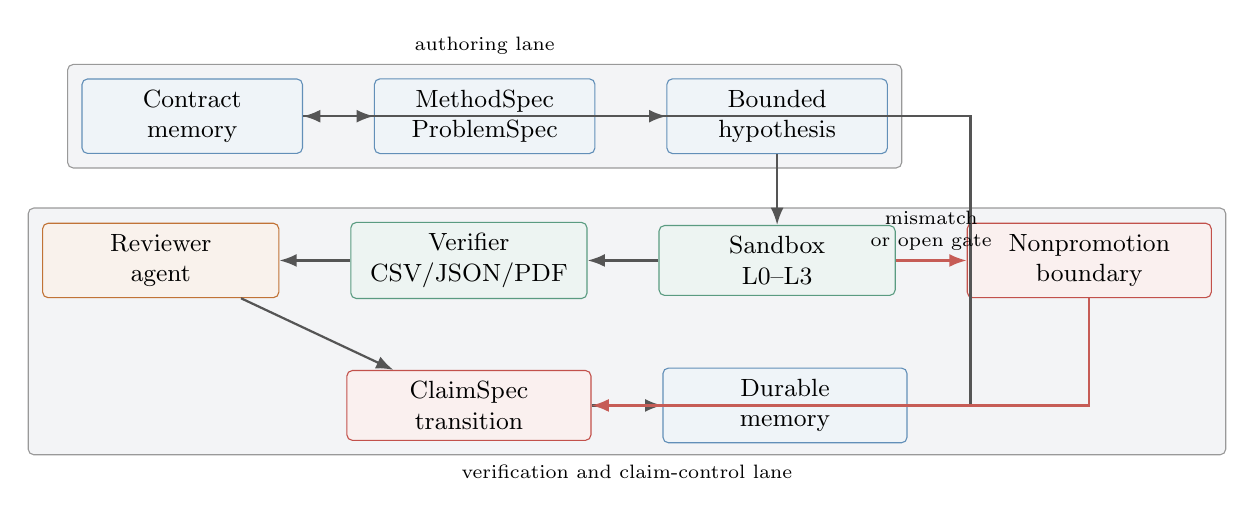
\begin{tikzpicture}[node distance=9mm and 9mm]
\node[paperbox, minimum width=28mm] (contract) {Contract\\memory};
\node[paperbox, right=of contract, minimum width=28mm] (method) {MethodSpec\\ProblemSpec};
\node[paperbox, right=of method, minimum width=28mm] (hyp) {Bounded\\hypothesis};
\node[verifierbox, below=of hyp, minimum width=30mm] (sandbox) {Sandbox\\L0--L3};
\node[verifierbox, left=of sandbox, minimum width=30mm] (verifier) {Verifier\\CSV/JSON/PDF};
\node[warningbox, left=of verifier, minimum width=30mm] (review) {Reviewer\\agent};
\node[boundarybox, below=of verifier, minimum width=31mm] (claim) {ClaimSpec\\transition};
\node[paperbox, right=of claim, minimum width=31mm] (memory) {Durable\\memory};
\node[boundarybox, right=of sandbox, minimum width=31mm] (block) {Nonpromotion\\boundary};

\draw[paperarrow] (contract) -- (method);
\draw[paperarrow] (method) -- (hyp);
\draw[paperarrow] (hyp) -- (sandbox);
\draw[paperarrow] (sandbox) -- (verifier);
\draw[paperarrow] (verifier) -- (review);
\draw[paperarrow] (review) -- (claim);
\draw[paperarrow] (claim) -- (memory);
\draw[paperarrow] (memory.east) -- ++(8mm,0) |- (contract.east);
\draw[claimarrow] (sandbox) -- node[above, font=\scriptsize, align=center]{mismatch\\or open gate} (block);
\draw[claimarrow] (block) |- (claim);

\begin{scope}[on background layer]
\node[lane, fit=(contract)(method)(hyp), label={[font=\scriptsize]above:authoring lane}] {};
\node[lane, fit=(sandbox)(verifier)(review)(claim)(block), label={[font=\scriptsize]below:verification and claim-control lane}] {};
\end{scope}
\end{tikzpicture}}
\caption{The method architecture becomes a verifier target. The agent must
keep the residual, proof boundary, validators, and artifact layer synchronized
instead of treating the implementation as an opaque script.}
\label{fig:method_architecture}
\end{figure}

\subsection{Claim state machine}

Each claim is assigned one of five states:
\begin{description}
  \item[Hypothesis.] A candidate method, repair, or comparison idea that has not
  yet passed a gate.
  \item[Diagnostic.] Evidence that is useful for understanding the system but
  not sufficient for a paper claim.
  \item[Accepted.] A claim whose required validators and ledgers agree.
  \item[Open.] A known blocker remains active.
  \item[Forbidden.] The wording conflicts with the current gate state and must
  be removed or demoted.
\end{description}
The important feature is reversibility. A claim can move backward when a
validator exposes stale prose, a mismatched reference policy, or a proof
obligation that was previously hidden.

\section{Verifier Sandbox}

The verifier sandbox constrains what the agent can run and what the resulting
output is allowed to mean. Four levels are used:

\begin{table}[H]
\centering
\caption{Verifier sandbox levels.}
\label{tab:sandbox}
\begin{tabularx}{\linewidth}{p{0.08\linewidth}p{0.24\linewidth}YY}
\toprule
\textbf{Level} & \textbf{Sandbox} & \textbf{Allowed question} & \textbf{Forbidden by default} \\
\midrule
L0 & Read-only validators & Do current claims match current artifacts? & Regenerating results or changing status. \\
L1 & Target audit & Can one bounded hypothesis falsify a local gap? & Promoting claims or rewriting ledgers. \\
L2 & Full generator & After method-code changes, do version-wide artifacts regenerate? & Using stale ledgers after regeneration. \\
L3 & External source-policy campaign & Do public same-test rows close under explicit policy? & Running expensive or policy-sensitive campaigns without opt-in. \\
\bottomrule
\end{tabularx}
\end{table}

This structure matters because different questions have different blast
radii. A paper-editing question should usually be answered by a read-only
validator, not by rerunning a full historical generator. A source-policy
external campaign can be expensive, and its results affect paper-level claims;
it should require explicit human opt-in. Conversely, after method code is
changed, a full artifact generator may be necessary because old summaries are
no longer authoritative.

At each level, the verifier has a different definition of success. A useful
agent must keep these definitions separate, because a pass at one level does
not imply a pass at another level.

\begin{table}[H]
\centering
\caption{Step-level verifier outputs and nonclaims.}
\label{tab:step_verifiers}
\small
\begin{tabularx}{\linewidth}{p{0.12\linewidth}p{0.29\linewidth}p{0.25\linewidth}Y}
\toprule
\textbf{Step} & \textbf{Verifier output} & \textbf{Claim it can support} & \textbf{Claim it cannot support} \\
\midrule
Contract audit & Accepted method name, order claim, open caveats, and stale tokens & Paper prose matches current artifacts & Numerical correctness or theorem closure \\
Method audit & Residual-row count, endpoint map, solver policy, and stage variables & The implementation is the intended candidate & Error order or external superiority \\
Example audit & Mechanism parameters, drivers, step sizes, references, and metrics & The benchmark is reproducible & Method superiority across papers \\
Convergence audit & Error table and observed slopes from at least three step sizes & Local asymptotic evidence under the stated reference & A theorem unless proof conditions are closed \\
Proof audit & Closed lemmas, retained assumptions, row certificates, and theorem interface & Conditional theorem statement with explicit assumptions & Empirical validation of open assumptions \\
Source-policy audit & Matched public parameters, references, work metrics, and runner status & Same-test readiness or completed same-test rows & External superiority if the campaign is not run \\
\bottomrule
\end{tabularx}
\end{table}

In the case study, the sandbox prevents three concrete mistakes. First,
endpoint projection evidence is kept separate from raw residual and KKT
closure evidence. Second, full-TFE replacement scans remain diagnostic until
they close the appropriate residual-substitution and order gates. Third,
v048 same-test scaffolds do not promote external-superiority claims until the
source-policy campaign is actually run.

\begin{figure}[t]
\centering
\resizebox{0.92\linewidth}{!}{%
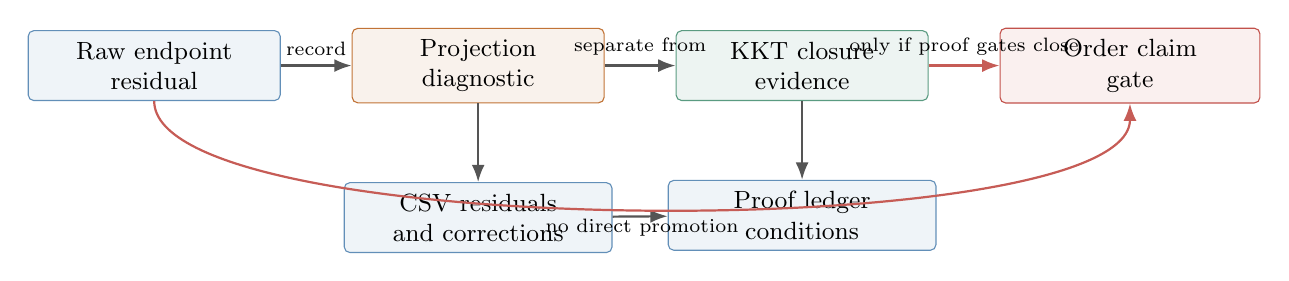
\begin{tikzpicture}[node distance=10mm and 9mm]
\node[paperbox, minimum width=32mm] (raw) {Raw endpoint\\residual};
\node[warningbox, right=of raw, minimum width=32mm] (proj) {Projection\\diagnostic};
\node[verifierbox, right=of proj, minimum width=32mm] (kkt) {KKT closure\\evidence};
\node[boundarybox, right=of kkt, minimum width=33mm] (claim) {Order claim\\gate};
\node[paperbox, below=of proj, minimum width=34mm] (csv) {CSV residuals\\and corrections};
\node[paperbox, below=of kkt, minimum width=34mm] (ledger) {Proof ledger\\conditions};

\draw[paperarrow] (raw) -- node[above, font=\scriptsize]{record} (proj);
\draw[paperarrow] (proj) -- node[above, font=\scriptsize]{separate from} (kkt);
\draw[claimarrow] (kkt) -- node[above, font=\scriptsize]{only if proof gates close} (claim);
\draw[paperarrow] (proj) -- (csv);
\draw[paperarrow] (kkt) -- (ledger);
\draw[paperarrow] (csv) -- (ledger);
\draw[claimarrow] (raw.south) .. controls +(0,-18mm) and +(0,-18mm) .. node[below, font=\scriptsize]{no direct promotion} (claim.south);
\end{tikzpicture}}
\caption{Endpoint closure is sandboxed as its own evidence stream. Projection,
raw residual, and KKT closure are recorded separately so that constraint repair
does not silently become an order claim.}
\label{fig:endpoint}
\end{figure}

\section{Proof Sandbox}

The proof sandbox specifies what may enter the theorem. For the \method{}
path, the current theorem-facing route is a conditional direct residual-bridge
route rather than a fully closed primitive Taylor-subterm route. The proof
ledger therefore records both accepted interfaces and retained conditions.

The theorem is decomposed around a one-step map. Let $\phi_h$ denote the exact
flow in a smooth reduced chart, $\Psi_h^G$ the ideal three-stage Gauss map, and
$\Psi_h^A$ the implemented \method{} map after stage residual, endpoint
closure, and inexact Newton effects. The proof target is not to show that every
piece of the implementation is symbolically identical to a source-paper TFE
residual. It is to show, under stated regularity and solver assumptions, that
the implemented map differs from the exact flow by a local defect of order
$h^7$:
\[
  \|\Psi_h^A(y)-\phi_h(y)\|
  \le
  C_G h^7 + C_A h^7 + C_E h^7 + C_N \eta_h .
\]
If the Newton tube tolerance satisfies $\eta_h \le c_{\eta} h^7$, then
\[
  \|\Psi_h^A(y)-\phi_h(y)\| \le
  C_{\mathrm{loc}} h^7,\qquad
  C_{\mathrm{loc}} = C_G + C_A + C_E + C_N c_{\eta}.
\]
One-step stability,
$\|\Psi_h(y)-\Psi_h(\bar y)\| \le (1+C_s h)\|y-\bar y\|$, then transfers the
local defect to a global sixth-order bound over $[0,T]$:
\[
  \max_{0\le n h\le T}\|y_n-y(t_n)\|
  \le C_{\mathrm{loc}}
  \frac{\exp(C_sT)-1}{C_s}\,h^6 .
\]
This is why the paper-facing claim is sixth order even when some smooth
observed slopes are higher. The observed slopes are evidence for the
implemented path; the theorem is bounded by the closed proof obligations.

\begin{table}[H]
\centering
\caption{Proof obligations tracked by the agent.}
\label{tab:proof}
\begin{tabularx}{\linewidth}{p{0.08\linewidth}YY}
\toprule
\textbf{ID} & \textbf{Obligation} & \textbf{Reason} \\
\midrule
P1 & Smooth reduced chart and FullVA lift & Gauss order must transfer through constrained coordinates. \\
P2 & Compact-tube branch, stage Jacobian, stability, and endpoint-closure interfaces & Newton and endpoint closure must define a local one-step map on the accepted branch. \\
P3 & Runtime formula and automatic-differentiation oracle for the 132-row residual & The implemented residual layout must be the residual being analyzed. \\
P4 & Non-dynamic $O(h^7)$ residual certificate and endpoint perturbation interface & The 96 non-dynamic rows and endpoint effects must not lower the local defect order. \\
P5 & Newton--Euler dynamic rows discharged by direct substitution & Dynamic force-balance rows cannot be hand-waved. \\
P6 & Solver residual $\eta_h \le c h^7$ & Fixed production tolerances are not theorem inputs. \\
P7 & Residual-to-error theorem for surrogate rows & Mechanism residual checks are not automatically order proofs. \\
\bottomrule
\end{tabularx}
\end{table}

The residual proof is then split by rows and by route. The current
implementation has a 132-row FullVA residual. The proof audit records a
96-row non-dynamic certificate and a 36-row dynamic Newton--Euler
direct-substitution check. These numbers matter because they prevent the
agent from writing ``all rows are symbolically proved'' when only a subset is
proved by a particular lane.

\begin{table}[H]
\centering
\caption{Residual-proof decomposition used by the agent.}
\label{tab:proof_rows}
\small
\begin{tabularx}{\linewidth}{p{0.18\linewidth}p{0.22\linewidth}p{0.21\linewidth}Y}
\toprule
\textbf{Block} & \textbf{Rows or interface} & \textbf{Current status} & \textbf{How the agent uses it} \\
\midrule
Non-dynamic residual certificate & 96 residual rows & Closed for the direct $O(h^7)$ certificate lane & Supports the implemented residual-defect block, not external comparison. \\
Dynamic Newton--Euler rows & 36 rows & Closed by direct substitution on the current route & Prevents dynamic force-balance rows from being treated as informal diagnostics. \\
P-interface assumptions & P1--P6 & Retained theorem conditions plus partial certificates & Defines the conditional theorem statement and prevents unconditional wording. \\
Residual-to-error bridge & P7 & Open & Keeps closed-loop four-link and slider-crank residual checks as coverage/consistency evidence. \\
Solver tolerance route & $\eta_h \le c_{\eta}h^7$ & Theorem condition retained; finite probes are diagnostics & Blocks fixed production tolerances from becoming proof-level closure. \\
\bottomrule
\end{tabularx}
\end{table}

\begin{algorithm}[H]
\caption{Proof-sandbox audit for the \method{} route}
\label{alg:proof_audit}
\begin{algorithmic}[1]
\Require 132-row residual implementation, proof ledger, Newton tolerance policy, ASME evidence rows
\Ensure Conditional theorem boundary and nonpromotion list
\State Verify that the runtime formula and AD oracle identify the same 132 residual rows
\State Check the 96 non-dynamic row certificate for $O(h^7)$ defect on the accepted lift
\State Check the 36 Newton--Euler rows by direct substitution on the current route
\State Retain P1/P2 compact-branch, smooth-lift, endpoint-closure, and stability assumptions
\State Retain P6 unless $\eta_h^{\mathrm{tube}}\le c_\eta h^7$ is proved as a theorem-level solver policy
\If{all local-defect blocks close under retained assumptions}
  \State allow the conditional local defect $O(h^7)$ and global sixth-order statement
\EndIf
\If{P7 residual-to-error obligations are not all closed}
  \State classify four-link/slider-crank residual rows as coverage and consistency only
\EndIf
\State Forbid unconditional theorem, source-policy superiority, and residual-to-error promotion
\end{algorithmic}
\end{algorithm}

\begin{figure}[H]
\centering
\resizebox{0.95\linewidth}{!}{%
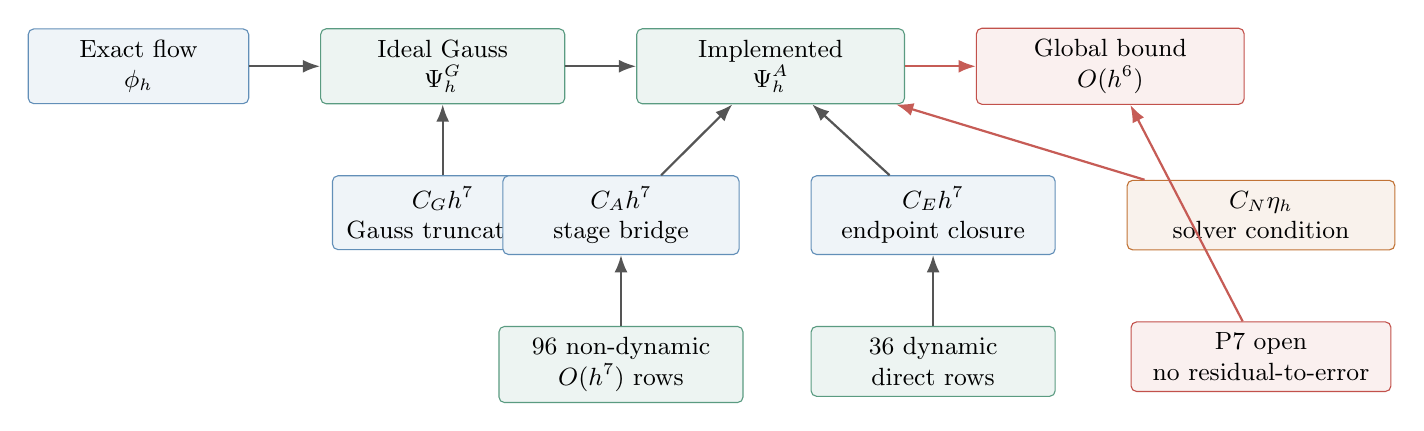
\begin{tikzpicture}[node distance=9mm and 9mm]
\node[paperbox, minimum width=28mm] (exact) {Exact flow\\$\phi_h$};
\node[verifierbox, right=of exact, minimum width=31mm] (gauss) {Ideal Gauss\\$\Psi_h^G$};
\node[verifierbox, right=of gauss, minimum width=34mm] (impl) {Implemented\\$\Psi_h^A$};
\node[boundarybox, right=of impl, minimum width=34mm] (global) {Global bound\\$O(h^6)$};

\node[paperbox, below=of gauss, minimum width=28mm] (cg) {$C_G h^7$\\Gauss truncation};
\node[paperbox, below=of impl, xshift=-19mm, minimum width=30mm] (ca) {$C_A h^7$\\stage bridge};
\node[paperbox, right=of ca, minimum width=31mm] (ce) {$C_E h^7$\\endpoint closure};
\node[warningbox, right=of ce, minimum width=34mm] (cn) {$C_N\eta_h$\\solver condition};
\node[verifierbox, below=of ca, minimum width=31mm] (rows96) {96 non-dynamic\\$O(h^7)$ rows};
\node[verifierbox, below=of ce, minimum width=31mm] (rows36) {36 dynamic\\direct rows};
\node[boundarybox, below=of cn, minimum width=33mm] (p7) {P7 open\\no residual-to-error};

\draw[paperarrow] (exact) -- (gauss);
\draw[paperarrow] (gauss) -- (impl);
\draw[claimarrow] (impl) -- (global);
\draw[paperarrow] (cg) -- (gauss);
\draw[paperarrow] (ca) -- (impl);
\draw[paperarrow] (ce) -- (impl);
\draw[claimarrow] (cn) -- (impl);
\draw[paperarrow] (rows96) -- (ca);
\draw[paperarrow] (rows36) -- (ce);
\draw[claimarrow] (p7) -- (global);
\end{tikzpicture}}
\caption{Proof sandbox decomposition. The conditional theorem route is built
from local-defect blocks and row certificates, while P7 prevents closed-loop
residual diagnostics from becoming trajectory-order proof.}
\label{fig:proof_decomposition}
\end{figure}

The P7 boundary is especially important for the four-link and slider-crank
examples. The proof contract records seven obligations that must close before
closed-loop reaction residuals can be used as trajectory-error or order proof:

\begin{table}[H]
\centering
\caption{Open residual-to-error obligations for P7.}
\label{tab:p7_obligations}
\small
\begin{tabularx}{\linewidth}{p{0.08\linewidth}Y}
\toprule
\textbf{ID} & \textbf{Blocking obligation} \\
\midrule
P7.1 & Dynamic residual identity. \\
P7.2 & Residual consistency rate $O(h^7)$. \\
P7.3 & Closed-loop DAE stability or inf--sup bound. \\
P7.4 & Calibrated non-floor-limited residual-to-error estimator. \\
P7.5 & Reference-floor exclusion. \\
P7.6 & Coarse-first accepted dynamic-order campaign. \\
P7.7 & Manuscript theorem and proof. \\
\bottomrule
\end{tabularx}
\end{table}

The ledger separates an accepted lane from a diagnostic lane. Accepted evidence
includes direct residual bridge checks, automatic-differentiation-expanded row
identities, and Newton--Euler direct-substitution certificates for the current
conditional route. Diagnostic evidence includes primitive Taylor fragments,
fixed-tolerance logs, residual-only closed-loop rows, and external
source-policy rows. This separation is essential because numerical evidence
can support a theorem but cannot substitute for a theorem condition.

\section{Numerical Example Ladder}

The agent chooses numerical examples by the failure mode they expose. The
ladder used in the case study is:

\begin{enumerate}
  \item SO(3) kinematics: right-action, chart, and log-map checks.
  \item Smooth mechanics: invariants and high-order smooth behavior.
  \item Constrained DAEs: position, velocity, and acceleration closure.
  \item Friction regimes: regularization width, pre-asymptotic order, and
  cost-to-recover order.
  \item ASME mechanisms: single pendulum, double pendulum, four-link, and
  slider-crank lower-pair coverage.
  \item External same-test baselines: matched parameters, references, errors,
  and work metrics.
\end{enumerate}

The ladder prevents premature promotion. The agent should not jump from a toy
kinematics plot to a paper claim about lower-pair multibody dynamics. Nor
should it use a closed-loop residual row as an external dynamic-order row until
the missing residual-to-error or same-test campaign is closed.

\section{Four ASME Example Protocols}
\label{sec:asme_protocols}

The four ASME-style examples are not decorative demonstrations. They are
verifiers with different jobs. The agent therefore stores, for each example,
the mechanism definition, the reference policy, the error norm, the order
formula, and the allowed claim state. This is the part of the workflow that
prevents a visually plausible mechanism animation from being overinterpreted
as a method-order theorem.

\subsection{Metric and reference policies}

The examples do not share one universal error metric. The agent instead
records the metric with the artifact that produced it. This is a critical
detail because the v047 closed-loop kinematic/reaction rows and the later
common-reference result matrix answer different questions.

\begin{table}[H]
\centering
\caption{Metric policies for ASME-related artifacts.}
\label{tab:metric_policies}
\small
\begin{tabularx}{\linewidth}{p{0.22\linewidth}p{0.24\linewidth}p{0.25\linewidth}Y}
\toprule
\textbf{Artifact lane} & \textbf{Reference and steps} & \textbf{Metric} & \textbf{Allowed use} \\
\midrule
Single-pendulum analytic method row & Analytic driven-angle reference; local method sweep $h=\{0.20,0.10,0.05\}$ over $T=0.2$ & Position/velocity, orientation-log, and angular-velocity errors from the method CSV & Accepted local method-side dynamic-order evidence. \\
Double-pendulum local method row & Nested local \method{} reference $h=0.005$; tested $h=\{0.04,0.02,0.01\}$ over $T=0.2$ & Orientation and angular-velocity errors plus constraint residual diagnostics & Accepted local method-side dynamic-order evidence under the local reference policy. \\
Closed-loop kinematic/reaction rows & Local kinematic FullVA reference $h=0.001$; tested $h=\{0.02,0.01,0.005\}$ over $T=0.2$ & Trajectory $L_\infty$ consistency, constraint residuals, multiplier reconstruction, Newton--Euler residuals & Four-link/slider-crank mechanism coverage and consistency only. The near-floor slopes are not dynamic-order claims. \\
Common-reference result matrix & Common diagnostic sweep $h=\{0.1,0.05,0.025\}$ with reference $h=0.0125$ & Recorded \texttt{final\_l2} or \texttt{final\_linf}; each cell reports observed order / finest-step error & Bounded common-reference diagnostic. It is not source-policy external superiority. \\
\bottomrule
\end{tabularx}
\end{table}

Within any one lane, the observed order is computed only from errors produced
under that same lane's reference and metric. With three nested step sizes
$h_0,h_1,h_2$ satisfying $h_{i+1}=h_i/2$, the agent records the log--log slope
\[
  \widehat p
  =
  \frac{\log(e_{h_0}/e_{h_2})}{\log(h_0/h_2)} ,
\]
with pairwise slopes and reference-floor warnings retained as diagnostics.
If the finest errors are at roundoff or reference-floor level, the row is not
promoted to an asymptotic order claim even if the formal slope is high.
Constraint residuals and Newton--Euler residuals are stored separately; they
are consistency diagnostics unless the residual-to-error theorem closes.

\begin{algorithm}[H]
\caption{Constructing one numerical evidence row}
\label{alg:evidence_row}
\begin{algorithmic}[1]
\Require Example $m$, method candidate, lane policy $\ell$, step list $H$, reference policy $r$, metric $d$
\Ensure Evidence row with errors, observed order, diagnostics, and claim scope
\State Load mechanism parameters, joints, drivers, initial state, horizon, and tolerances for $m$
\State Generate or load the reference trajectory/state according to $r$
\For{each $h \in H$}
  \State Run the method under the lane policy $\ell$
  \State Compute the lane-specific error $e_h=d(y_h,y_{\mathrm{ref}})$
  \State Record constraint residuals, Newton diagnostics, and reaction residuals separately
\EndFor
\State Compute $\widehat p=\log(e_{h_0}/e_{h_2})/\log(h_0/h_2)$ and pairwise slopes
\If{reference floor, nonmonotonic errors, or open P7/source-policy gate is detected}
  \State mark the row as diagnostic or coverage-only
\Else
  \State mark the row as accepted for the specific ClaimSpec it satisfies
\EndIf
\State Write CSV/JSON/table entries with the reference, metric, finest error, order, and claim scope
\end{algorithmic}
\end{algorithm}

\begin{table}[H]
\centering
\caption{Protocol summary for the four ASME examples and their evidence lanes.}
\label{tab:asme_protocols}
\small
\begin{tabularx}{\linewidth}{p{0.15\linewidth}p{0.26\linewidth}p{0.25\linewidth}Y}
\toprule
\textbf{Example} & \textbf{Mechanism and reference} & \textbf{Compared quantities} & \textbf{Allowed interpretation} \\
\midrule
Single pendulum & Driven ASME single pendulum; analytic driven-angle reference; $T=0.2$, method-row $h=\{0.20,0.10,0.05\}$ and common-matrix $h=\{0.1,0.05,0.025\}$. & COM position/velocity, orientation log error, angular velocity, drive residual diagnostics, and final-error matrix row. & Accepted local method-side dynamic-order evidence; external rows remain diagnostics unless source-policy closes. \\
Double pendulum & Two-revolute ASME double pendulum mapped to the FullVA side method; nested local reference $h=0.005$ for method row; common-matrix reference $h=0.0125$. & Orientation and angular velocity errors plus position-, velocity-, and acceleration-level constraint residuals. & Accepted local method-side dynamic-order evidence under the local reference policy; external rA comparison remains pending. \\
Four-link local coverage & Driven closed-loop mechanism with 18 generalized coordinates and 18 constraints; local kinematic FullVA reference $h=0.001$; $h=\{0.02,0.01,0.005\}$. & Trajectory $L_\infty$ consistency, constraint residuals, and reconstructed Newton--Euler reaction residuals. & Mechanism coverage and closed-loop consistency, not accepted dynamic-order proof. \\
Four-link common-reference diagnostic & Same mechanism in the paper result matrix; reference $h=0.0125$; $h=\{0.1,0.05,0.025\}$. & \texttt{final\_linf} position/velocity/acceleration errors reported as order / finest-step error. & Internal common-reference diagnostic; not a source-policy or residual-to-error promotion. \\
Slider-crank local coverage & Closed-loop slider-crank with DP1, DP2, coordinate-difference, and distance constraints; local kinematic FullVA reference $h=0.001$; $h=\{0.02,0.01,0.005\}$. & Trajectory $L_\infty$ consistency, multiplier reconstruction, and translational/rotational dynamic residuals. & Mechanism coverage and closed-loop consistency, not accepted dynamic-order proof. \\
Slider-crank common-reference diagnostic & Same mechanism in the paper result matrix; reference $h=0.0125$; $h=\{0.1,0.05,0.025\}$. & \texttt{final\_linf} position/velocity/acceleration errors reported as order / finest-step error. & Internal common-reference diagnostic; not external superiority and not residual-to-error closure. \\
\bottomrule
\end{tabularx}
\end{table}

\begin{table}[H]
\centering
\caption{Numerical evidence rows for the four ASME examples in the common-reference matrix.}
\label{tab:asme_numeric_rows}
\scriptsize
\begin{tabularx}{\linewidth}{>{\raggedright\arraybackslash}p{0.13\linewidth}>{\raggedright\arraybackslash}p{0.24\linewidth}>{\raggedright\arraybackslash}p{0.23\linewidth}>{\raggedright\arraybackslash}p{0.15\linewidth}Y}
\toprule
\textbf{Example} & \textbf{Reference, metric, and sweep} & \textbf{Position/velocity order and finest error} & \textbf{Acceleration row} & \textbf{Claim scope} \\
\midrule
Single pendulum & Analytic driven-angle reference; \texttt{final\_l2}; $h=\{0.1,0.05,0.025\}$. & Position: $6.013$ / $3.323{\times}10^{-14}$. Velocity: $5.801$ / $1.155{\times}10^{-12}$. & Not a promoted matrix claim. & Consistent with the accepted local dynamic-order row; not external superiority. \\
Double pendulum & Local \method{} final-state reference at $h=0.0125$; \texttt{final\_linf}; same sweep. & Position: $6.011$ / $3.100{\times}10^{-13}$. Velocity: $6.010$ / $2.346{\times}10^{-13}$. & Not a promoted matrix claim. & Common-reference diagnostic plus accepted local dynamic-order row under its own reference policy. \\
Four-link & Closed-loop endpoint reference at $h=0.0125$; \texttt{final\_linf}; same sweep. & Position: $5.955$ / $2.289{\times}10^{-12}$. Velocity: $6.085$ / $1.093{\times}10^{-11}$. & $0.995$ / $8.80{\times}10^{-1}$. & Coverage and consistency only; P7 blocks dynamic-order promotion. \\
Slider-crank & Closed-loop endpoint reference at $h=0.0125$; \texttt{final\_linf}; same sweep. & Position: $6.164$ / $8.583{\times}10^{-12}$. Velocity: $7.341$ / $9.189{\times}10^{-12}$. & $1.054$ / $1.04{\times}10^{-1}$. & Coverage and consistency only; P7 blocks dynamic-order promotion. \\
\bottomrule
\end{tabularx}
\end{table}

\begin{figure}[H]
\centering
\resizebox{0.95\linewidth}{!}{%
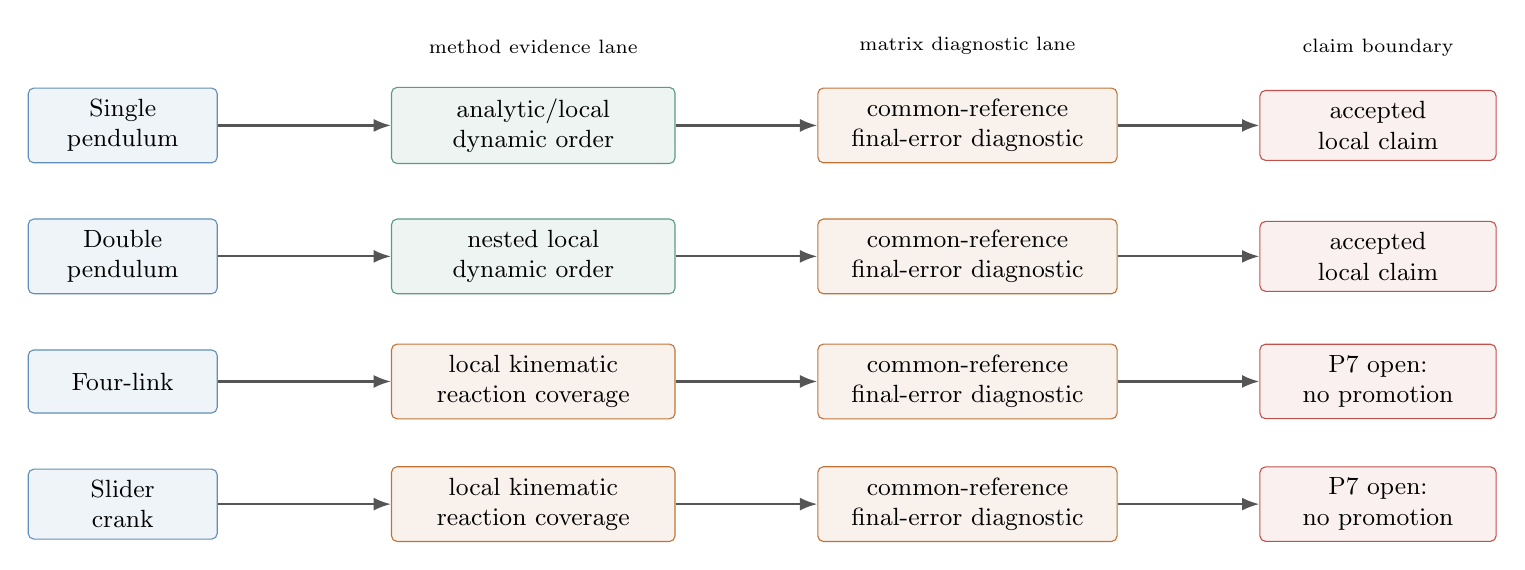
\begin{tikzpicture}[node distance=7mm and 7mm]
\node[paperbox, minimum width=24mm] (single) {Single\\pendulum};
\node[paperbox, below=of single, minimum width=24mm] (double) {Double\\pendulum};
\node[paperbox, below=of double, minimum width=24mm] (four) {Four-link};
\node[paperbox, below=of four, minimum width=24mm] (slider) {Slider\\crank};

\node[verifierbox, right=22mm of single, minimum width=36mm] (dyn1) {analytic/local\\dynamic order};
\node[verifierbox, right=22mm of double, minimum width=36mm] (dyn2) {nested local\\dynamic order};
\node[warningbox, right=22mm of four, minimum width=36mm] (cov1) {local kinematic\\reaction coverage};
\node[warningbox, right=22mm of slider, minimum width=36mm] (cov2) {local kinematic\\reaction coverage};

\node[warningbox, right=18mm of dyn1, minimum width=38mm] (mat1) {common-reference\\final-error diagnostic};
\node[warningbox, right=18mm of dyn2, minimum width=38mm] (mat2) {common-reference\\final-error diagnostic};
\node[warningbox, right=18mm of cov1, minimum width=38mm] (mat3) {common-reference\\final-error diagnostic};
\node[warningbox, right=18mm of cov2, minimum width=38mm] (mat4) {common-reference\\final-error diagnostic};

\node[boundarybox, right=18mm of mat1, minimum width=30mm] (claim1) {accepted\\local claim};
\node[boundarybox, right=18mm of mat2, minimum width=30mm] (claim2) {accepted\\local claim};
\node[boundarybox, right=18mm of mat3, minimum width=30mm] (claim3) {P7 open:\\no promotion};
\node[boundarybox, right=18mm of mat4, minimum width=30mm] (claim4) {P7 open:\\no promotion};

\foreach \a/\b in {single/dyn1,double/dyn2,four/cov1,slider/cov2,dyn1/mat1,dyn2/mat2,cov1/mat3,cov2/mat4,mat1/claim1,mat2/claim2,mat3/claim3,mat4/claim4}
  \draw[paperarrow] (\a) -- (\b);
\node[font=\scriptsize, above=3mm of dyn1] {method evidence lane};
\node[font=\scriptsize, above=3mm of mat1] {matrix diagnostic lane};
\node[font=\scriptsize, above=3mm of claim1] {claim boundary};
\end{tikzpicture}}
\caption{ASME evidence lanes. The examples share a result matrix but do not
share the same claim status: single and double support local dynamic-order
evidence, while four-link and slider-crank remain coverage/consistency until
P7 closes.}
\label{fig:asme_evidence_lanes}
\end{figure}

\subsection{Single pendulum}

The single-pendulum example is the cleanest dynamic-order verifier because the
drive provides an analytic reference. The public mechanism uses a length
$4\,\mathrm{m}$ body, square side length $0.05\,\mathrm{m}$, density
$7800\,\mathrm{kg/m^3}$, gravity $9.81\,\mathrm{m/s^2}$, and a DP1 drive of
the form
\[
  \cos\!\left(\frac{\pi}{2}+\frac{\pi}{4}\cos(2t)\right).
\]
The local \method{} row solves right-Lie orientation increments together with
center-of-mass position, velocity, acceleration, angular velocity, angular
acceleration, pivot reaction, axis multipliers, and drive multiplier. The
residual includes pivot position, pivot velocity, pivot acceleration,
revolute-axis DP1 rows, and acceleration-level drive closure.

The reference is the analytic driven angle and its derivatives, sampled on
the same grid as the numerical result. The primary comparisons are position,
velocity, orientation, and angular velocity. In the current accepted row, the
three-step sweep reports observed orders approximately $6.073$ for position,
$6.033$ for velocity, $6.055$ for orientation, and $6.024$ for angular
velocity. This is why the row supports the local sixth-order method claim.

\subsection{Double pendulum}

The double-pendulum row tests whether the FullVA mechanism survives a genuine
two-joint coupled system. The ASME mechanism has two bodies of lengths
$4\,\mathrm{m}$ and $2\,\mathrm{m}$, square side length $0.05\,\mathrm{m}$,
density $7800\,\mathrm{kg/m^3}$, gravity $9.81\,\mathrm{m/s^2}$, and two
revolute joints. The local mapping uses the v029-style double-revolute
\method{} side method. Public zero initial angular speeds are regularized by
opposite $10^{-12}$ perturbations to avoid a singular local convention; this
regularization is recorded as part of the ProblemSpec and is not hidden.

The reference is a nested local \method{} trajectory at $h=0.005$, while the
tested step sizes are $h=\{0.04,0.02,0.01\}$ over $T=0.2$. The accepted
comparisons are orientation and angular velocity errors, with constraint
residuals retained as consistency checks. The current row reports observed
orders approximately $6.101$ for orientation and $6.089$ for angular velocity.
This is accepted method-side dynamic-order evidence, but it is not yet a
same-test public rA superiority claim because the public-source reference and
work-policy campaign is a separate v048 gate.

\subsection{Four-link}

The four-link row is deliberately tagged differently. The mechanism has three
moving bodies with masses $2,1,1$ and inertias
$(4,2,0)$, $(12.4,0.01,0)$, and $(4.54,0.01,0)$ under the local convention.
The driver is $\cos(\pi t+\pi/2)$. The local closed-loop kinematic FullVA
system uses 18 generalized coordinates and 18 constraints, including six DP1
rows and twelve coordinate-difference rows. The recorded minimum singular
value of the kinematic constraint Jacobian is about $7.92\times10^{-2}$, with
condition number about $1.17\times10^2$.

The v047 local coverage reference is a kinematic FullVA trajectory at
$h=0.001$, while the coverage sweep uses $h=\{0.02,0.01,0.005\}$ over $T=0.2$.
That sweep is a nested sampling and reproducibility check: the recorded
trajectory errors are near the reference floor and the formal slopes are not
interpreted as dynamic order. A separate multiplier reconstruction checks
\[
  \Phi_q^\top \lambda =
  \begin{bmatrix}
  F-Ma\\
  -\bigl(J\alpha+\omega\times J\omega\bigr)
  \end{bmatrix},
\]
and records Newton--Euler residuals around $10^{-13}$. This supports
closed-loop consistency, not an external-order claim.

The paper result matrix has a separate common-reference diagnostic lane for
the same mechanism. There, the local \method{} row uses
$h=\{0.1,0.05,0.025\}$, reference $h=0.0125$, and \texttt{final\_linf}
errors. That lane reports position/velocity slopes about $5.955$ and $6.085$
with finest position/velocity errors about $2.289\times 10^{-12}$ and
$1.093\times 10^{-11}$. Because this lane is a common-reference diagnostic and
because P7 remains open, those slopes are not promoted into closed-loop
dynamic-order proof.

\subsection{Slider-crank}

The slider-crank example stresses mixed lower-pair constraints. The public
mechanism distinguishes the 2021 and 2022 parameter policies; the local
2021-style row uses masses $0.12$, $0.5$, and $2$ with inertias
$(10^{-4},10^{-5},10^{-4})$, $(4\times10^{-3},4\times10^{-4},4\times10^{-3})$,
and $(10^{-4},10^{-4},10^{-4})$. The driver is
$\cos(-2\pi t+\pi/2)$. The local constraint inventory includes seven DP1
rows, four DP2 rows, six coordinate-difference rows, and one distance row,
with a recorded minimum singular value about $7.25\times10^{-2}$ and
condition number about $43.6$.

As in the four-link case, the v047 local coverage reference is a kinematic
FullVA trajectory at $h=0.001$ with $h=\{0.02,0.01,0.005\}$ over $T=0.2$.
Those local kinematic rows record near-floor trajectory and constraint
consistency; they are not the source of a dynamic-order claim. The
reconstructed reaction-dynamics residuals are near $6\times10^{-15}$ across
the sweep.

The result matrix again contains a separate common-reference diagnostic lane
with $h=\{0.1,0.05,0.025\}$, reference $h=0.0125$, and \texttt{final\_linf}
errors. That lane reports position/velocity slopes about $6.164$ and $7.341$
with finest position/velocity errors about $8.583\times10^{-12}$ and
$9.189\times10^{-12}$. The acceleration slope is not used as a method-order
claim because the acceleration column is dominated by reconstruction and
floor behavior. The correct paper wording is therefore ``slider-crank
closed-loop coverage plus common-reference diagnostics,'' not ``accepted
slider-crank dynamic sixth-order proof'' and not ``public baseline
superiority.''

\section{Versioned Case Study: v001 to v048}

The version history is the strongest evidence that the agent must be
domain-specific. The versions are not a changelog; they are a record of
blockers. Each phase added a verifier because the previous phase exposed a new
way an integrator could fail.

The baseline before v001 was a conventional research workflow: implement a
candidate formula, run a small number of scripts, inspect convergence plots,
and then summarize the result in prose. That workflow is adequate for many
ordinary software experiments, but it breaks down for this project because the
same word ``method'' can hide different residuals, endpoint policies,
reference solutions, and proof assumptions. The shift from the baseline to
v001 was therefore not merely the creation of a first script. It was the first
attempt to make method identity auditable. The shift from v001 to the current
v048 endpoint was then driven by successive discoveries that a new piece of
the research state had to be made explicit.

\begin{table}[H]
\centering
\caption{Blocker-driven evolution of the research pipeline.}
\label{tab:evolution}
\begin{tabularx}{\linewidth}{p{0.18\linewidth}p{0.25\linewidth}Y}
\toprule
\textbf{Versions} & \textbf{Phase} & \textbf{Why the project evolved} \\
\midrule
v001--v005 & Lie-group basics & Establish SO(3) order, right-action conventions, and smooth Gauss mechanics before adding constraints. \\
v006--v013 & Constrained DAE closure & Endpoint position, velocity, and acceleration consistency became explicit verifier targets. \\
v014--v022 & Friction regimes & Sharp regularized friction exposed delayed asymptotic behavior and cost-to-recover-order questions. \\
v023--v029 & FullVA emergence & Absolute-coordinate lower-pair attempts exposed endpoint velocity/acceleration consistency failures. \\
v030--v045 & Solver scaling & Dense Jacobians and dense solves became bottlenecks, so sparse pattern and coloring audits became separate claims. \\
v046--v048 & Claim gates and external policy & ASME examples, proof ledgers, paper packages, and same-test scaffolds became first-class objects. \\
\bottomrule
\end{tabularx}
\end{table}

\begin{figure}[H]
\centering
\resizebox{\linewidth}{!}{%
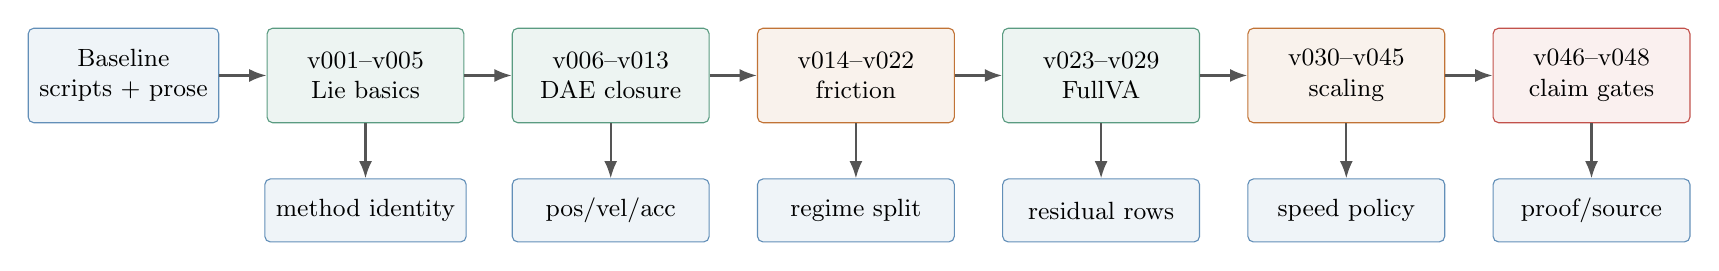
\begin{tikzpicture}[node distance=7mm and 6mm]
\node[paperbox, minimum width=24mm, minimum height=12mm] (base) {Baseline\\scripts + prose};
\node[verifierbox, right=of base, minimum width=25mm, minimum height=12mm] (lie) {v001--v005\\Lie basics};
\node[verifierbox, right=of lie, minimum width=25mm, minimum height=12mm] (dae) {v006--v013\\DAE closure};
\node[warningbox, right=of dae, minimum width=25mm, minimum height=12mm] (fric) {v014--v022\\friction};
\node[verifierbox, right=of fric, minimum width=25mm, minimum height=12mm] (fullva) {v023--v029\\FullVA};
\node[warningbox, right=of fullva, minimum width=25mm, minimum height=12mm] (scale) {v030--v045\\scaling};
\node[boundarybox, right=of scale, minimum width=25mm, minimum height=12mm] (claims) {v046--v048\\claim gates};

\node[paperbox, below=of lie, minimum width=25mm] (g1) {method identity};
\node[paperbox, below=of dae, minimum width=25mm] (g2) {pos/vel/acc};
\node[paperbox, below=of fric, minimum width=25mm] (g3) {regime split};
\node[paperbox, below=of fullva, minimum width=25mm] (g4) {residual rows};
\node[paperbox, below=of scale, minimum width=25mm] (g5) {speed policy};
\node[paperbox, below=of claims, minimum width=25mm] (g6) {proof/source};

\draw[paperarrow] (base) -- (lie);
\draw[paperarrow] (lie) -- (dae);
\draw[paperarrow] (dae) -- (fric);
\draw[paperarrow] (fric) -- (fullva);
\draw[paperarrow] (fullva) -- (scale);
\draw[paperarrow] (scale) -- (claims);
\draw[paperarrow] (lie) -- (g1);
\draw[paperarrow] (dae) -- (g2);
\draw[paperarrow] (fric) -- (g3);
\draw[paperarrow] (fullva) -- (g4);
\draw[paperarrow] (scale) -- (g5);
\draw[paperarrow] (claims) -- (g6);
\end{tikzpicture}}
\caption{Version evolution as a sequence of forced verifier additions. The
pipeline did not evolve because later versions were cosmetically cleaner; it
evolved because each phase exposed a new ambiguity that the agent had to make
auditable.}
\label{fig:version_evolution}
\end{figure}

\begin{table}[H]
\centering
\caption{Fine-grained evolution from baseline to the current v048 endpoint.}
\label{tab:version_detail}
\small
\begin{tabularx}{\linewidth}{p{0.13\linewidth}p{0.23\linewidth}p{0.28\linewidth}Y}
\toprule
\textbf{Stage} & \textbf{What was learned} & \textbf{Why the next stage was needed} & \textbf{Verifier added} \\
\midrule
Baseline & Public mechanisms, source-paper TFE ideas, and local scripts existed as separate objects. & The workflow could not distinguish formula comparison, source-code reproduction, and paper claim readiness. & Claim-state boundary and durable artifact memory. \\
v001 & First SO(3) benchmark suite gave a controlled Lie-group kinematics baseline. & Correct SO(3) motion was necessary but not enough; action convention and chart choice could silently change the method. & Right-action and log-map orientation checks. \\
v002--v005 & CF4/RKMK4 repairs, SBEL rA reproduction, Yoshida midpoint, and Gauss-Lie4 smooth mechanics clarified fourth-order behavior. & Smooth unconstrained order did not test DAE closure, lower-pair constraints, or endpoint velocity/acceleration consistency. & Smooth mechanics convergence and invariant checks. \\
v006--v008 & Fixed-pivot and absolute-coordinate DAE experiments showed that position closure alone was insufficient. & Endpoint constraints had to include position, velocity, and acceleration levels, otherwise projections could mask method drift. & Position/velocity/acceleration closure validators. \\
v009--v013 & Quaternion/JAX/Gauss6 variants achieved smooth high order but exposed sharp-friction order reduction. & The agent needed to separate smooth theorem evidence from nonsmooth or regularized-friction regimes. & Smooth-vs-sharp friction sweeps and cost-to-recover-order diagnostics. \\
v014--v022 & Brown--McPhee and revolute benchmark stages studied friction smoothness, adaptivity, and cost. & The next blocker was no longer scalar accuracy; it was lower-pair absolute-coordinate residual design. & Friction-width ledgers and benchmark-specific diagnostics. \\
v023--v029 & Full absolute revolute DAE attempts evolved toward Off-axis FullVA and double-revolute FullVA. & Endpoint velocity and acceleration consistency became the central method identity issue. & FullVA residual-row audits and double-revolute dynamic-order rows. \\
v030--v045 & Sparse CSR Newton, matrix-free attempts, lagging, colored JVP/VJP, symbolic pattern, and pattern cache studied scaling. & Exact sparsity did not imply runtime superiority; speed claims needed their own evidence policy. & Sparse-pattern certificates and dense-vs-sparse timing caveats. \\
v046--v047 & Four ASME examples, proof contracts, paper package, and claim audits were integrated. & The paper could now build mechanically, but source-policy and global submission-readiness claims were still open. & ASME result matrix, proof traceability audit, paper-claim audit. \\
v048 & Same-test external benchmark scaffold and public-code pilot rows were added. & External superiority still required matched public parameters, references, work metrics, and completed campaigns. & Cross-paper source-policy spec and opt-in external campaign gate. \\
\bottomrule
\end{tabularx}
\end{table}

\begin{table}[H]
\centering
\caption{Compact version ladder, v001--v012.}
\label{tab:version_ladder_a}
\scriptsize
\begin{tabularx}{\linewidth}{p{0.08\linewidth}p{0.37\linewidth}Y}
\toprule
\textbf{Version} & \textbf{Research turn} & \textbf{Verifier or claim-boundary effect} \\
\midrule
v001 & First reproducible SO(3) benchmark suite. & Created benchmark memory before high-order claims. \\
v002 & Corrected right-action CF4/RKMK4 fourth-order kinematics. & Made action convention and log-map order checks explicit. \\
v003 & Reproduced SBEL/Negrut rA code path. & Added a source-code reproducibility anchor, not a high-order claim. \\
v004 & Added Yoshida-composed Lie midpoint mechanics. & Recorded that negative substeps are poor for friction/contact. \\
v005 & Added two-stage Gauss-Lie4 smooth mechanics. & Established smooth unconstrained order and invariant checks. \\
v006 & Moved to reduced fixed-pivot DAE. & Separated exact reconstruction from full absolute-coordinate DAE. \\
v007 & Implemented absolute-coordinate Gauss DAE. & Exposed the need for position, velocity, and acceleration consistency. \\
v008 & Internalized endpoint constraints in the Newton solve. & Reduced reliance on endpoint projection. \\
v009 & Added smooth and sharp regularized friction. & Split smooth-order evidence from sharp-friction order reduction. \\
v010 & Replaced finite-difference Jacobians with JAX AD. & Made nonlinear-solve backend evidence a separate lane. \\
v011 & Implemented quaternion transport operators. & Bridged local SO(3) residuals to paper-style S3 transport. \\
v012 & Embedded quaternion endpoint DAE residual. & Verified quaternion residual identity before increasing order. \\
\bottomrule
\end{tabularx}
\end{table}

\begin{table}[H]
\centering
\caption{Compact version ladder, v013--v024.}
\label{tab:version_ladder_b}
\scriptsize
\begin{tabularx}{\linewidth}{p{0.08\linewidth}p{0.37\linewidth}Y}
\toprule
\textbf{Version} & \textbf{Research turn} & \textbf{Verifier or claim-boundary effect} \\
\midrule
v013 & Added Gauss6 endpoint collocation. & Produced sixth-order smooth evidence while preserving sharp-friction caveats. \\
v014 & Swept friction smoothness. & Turned ``Gauss6 is worth it'' into a regime-dependent claim. \\
v015 & Added adaptive Gauss6/Gauss4 controller. & Quantified near-nonsmooth cost/accuracy tradeoffs. \\
v016 & Added reduced Lie-trapezoidal baseline. & Ruled out a favorable low-order baseline as the main winner. \\
v017 & Added reduced Lie-BDF2 baseline. & Kept robustness evidence separate from accuracy leadership. \\
v018 & Tested Lobatto endpoint collocation. & Prevented simple TFE-style endpoint-node substitution from being overclaimed. \\
v019 & Added reaction-dependent friction. & Connected multiplier/reaction loads to the residual. \\
v020 & Added adaptive lambda-friction controller. & Quantified sharp lambda-friction recovery. \\
v021 & Added Brown--McPhee-style friction. & Moved from surrogate friction toward paper-like continuous friction. \\
v022 & Added revolute Brown--McPhee benchmark. & Made a paper-like one-DOF revolute friction verifier. \\
v023 & Built full absolute-coordinate revolute DAE. & Exposed endpoint velocity and formulation fragility. \\
v024 & Tried direct Lobatto full revolute DAE. & Recorded failure of simple Gauss-to-Lobatto node replacement. \\
\bottomrule
\end{tabularx}
\end{table}

\begin{table}[H]
\centering
\caption{Compact version ladder, v025--v036.}
\label{tab:version_ladder_c}
\scriptsize
\begin{tabularx}{\linewidth}{p{0.08\linewidth}p{0.37\linewidth}Y}
\toprule
\textbf{Version} & \textbf{Research turn} & \textbf{Verifier or claim-boundary effect} \\
\midrule
v025 & Added endpoint projection repair. & Separated practical constraint repair from unchanged one-step-map claims. \\
v026 & Added stage pivot-velocity residual. & Made velocity closure a residual-row target. \\
v027 & Added stage pivot-acceleration residual. & Made acceleration closure a residual-row target. \\
v028 & Added off-axis FullVA residual. & Checked axis velocity/acceleration consistency under off-axis torque. \\
v029 & Extended to double-revolute interbody system. & Showed FullVA generalizes and exposed sparse/block Newton needs. \\
v030 & Measured double-revolute Jacobian sparsity and CSR timing. & Turned solver scaling into a separate evidence lane. \\
v031 & Integrated CSR sparse solves into Newton. & Showed sparse solves preserve trajectory but still depend on dense AD materialization. \\
v032 & Tested JVP-GMRES matrix-free Newton. & Recorded matrix-free failure without preconditioning. \\
v033 & Tested lagged sparse Newton. & Recorded that reduced Jacobian refreshes did not materially improve runtime. \\
v034 & Tested colored-JVP sparse assembly. & Verified sparse AD correctness but rejected it as small-system speed winner. \\
v035 & Batched colored JVP seeds. & Improved sparse AD runtime while retaining exactness checks. \\
v036 & Generated block-symbolic sparse pattern. & Removed dense warm-up as the only pattern source. \\
\bottomrule
\end{tabularx}
\end{table}

\begin{table}[H]
\centering
\caption{Compact version ladder, v037--v048.}
\label{tab:version_ladder_d}
\scriptsize
\begin{tabularx}{\linewidth}{p{0.08\linewidth}p{0.37\linewidth}Y}
\toprule
\textbf{Version} & \textbf{Research turn} & \textbf{Verifier or claim-boundary effect} \\
\midrule
v037 & Pruned symbolic pattern with JVP dry-runs. & Recovered exact observed sparsity without dense Jacobian discovery. \\
v038 & Reused cached JVP-pruned pattern. & Added cache/reuse policy for nearby regimes. \\
v039 & Extended to triple-revolute topology. & Tested sparse AD beyond the two-body case. \\
v040 & Generated block pattern for triple revolute. & Made larger-topology pattern acquisition more production-like. \\
v041 & Added cache refresh/union policy. & Recorded stale-cache detection and refresh rules. \\
v042 & Added skew-axis triple-revolute lower pairs. & Tested non-coplanar lower-pair geometry. \\
v043 & Added skew prismatic lower pair. & Added non-revolute coverage while preserving sparse-speed caveat. \\
v044 & Added double-prismatic interbody chain. & Exposed high color count and dense-backend competitiveness. \\
v045 & Added row-colored VJP sparse AD. & Reduced seed count but retained dense-runtime caveat. \\
v046 & Validated upstream ASME rA examples. & Created four-example public/reproducibility anchor without a Gauss6 method claim. \\
v047 & Built cylindrical-chain \method{} pipeline and claim gates. & Integrated 132-row residual, proof audits, ASME evidence, smooth-order evidence, caveats, and paper-package validators. \\
v048 & Built same-test external benchmark harness. & Added public-code pilots and source-policy scaffolding while keeping external superiority false. \\
\bottomrule
\end{tabularx}
\end{table}

This evolution explains why the current agent records negative and partial
results instead of deleting them. v004 was useful because negative substeps
were poor for friction/contact. v013 was useful because the same Gauss6 path
showed smooth order near six but sharp-friction pre-asymptotic order around
the low-order regime. v030--v045 were useful because they showed that a
correct sparse pattern did not automatically beat a dense automatic
differentiation implementation. v048 is useful even though it does not close
external superiority, because it turns the public comparison into a structured
source-policy campaign rather than a prose-level aspiration.

\begin{table}[H]
\centering
\caption{Evidence-state matrix used by the agent.}
\label{tab:evidence_state_matrix}
\small
\begin{tabularx}{\linewidth}{p{0.18\linewidth}p{0.21\linewidth}p{0.21\linewidth}p{0.19\linewidth}Y}
\toprule
\textbf{Evidence lane} & \textbf{Single pendulum} & \textbf{Double pendulum} & \textbf{Four-link} & \textbf{Slider-crank} \\
\midrule
Local dynamic-order method row & Accepted; analytic/reference-policy order evidence & Accepted; nested local reference order evidence & Not used as local dynamic-order proof & Not used as local dynamic-order proof \\
Local kinematic/reaction coverage & Reaction reconstruction diagnostic & Constraint residual diagnostic & Accepted coverage and reaction consistency & Accepted coverage and reaction consistency \\
Common-reference result matrix & Internal order/error diagnostic & Internal order/error diagnostic & Internal final-error diagnostic only & Internal final-error diagnostic only \\
External source-policy claim & Open; no superiority claim & Open; no superiority claim & Open; no superiority claim & Open; no superiority claim \\
Proof promotion boundary & Conditional sixth-order method claim & Conditional sixth-order method claim & Blocked by P7 residual-to-error obligations & Blocked by P7 residual-to-error obligations \\
\bottomrule
\end{tabularx}
\end{table}

The evolution has two methodological implications. First, a version should be
created when the research question changes, not when a script is cosmetically
edited. Second, negative results are useful artifacts. A failed TFE replacement
candidate that records rank, residual, and missing span prevents the next agent
run from rediscovering the same failure.

\section{Current Evidence Boundary}

\subsection{Accepted local method evidence}

The current accepted local method object is the \method{} path. It has three
Gauss stages and 132 FullVA residual rows. The smooth cylindrical-chain
h-sweep records observed position/velocity orders about 7.161/7.066. The
paper-facing method claim is conditional sixth order, not seventh order, and
not full source-paper residual reproduction.

\begin{figure}[t]
\centering

\includegraphics[width=0.80\linewidth]{convergence.png}
\caption{Smooth convergence evidence for the current local \method{} path. The
observed slopes support the method evidence, while the theorem claim remains
bounded by the proof ledger.}
\label{fig:convergence}
\end{figure}

\subsection{ASME mechanism evidence}

The four ASME-style mechanisms enter the current method evidence system:
single pendulum, double pendulum, four-link, and slider-crank. The current
boundary distinguishes dynamic-order evidence from mechanism coverage. Single-
and double-pendulum rows support accepted method-side dynamic-order evidence.
Four-link and slider-crank rows support closed-loop kinematic FullVA coverage
and reaction-dynamics consistency; they are not promoted into accepted
asymptotic dynamic-order proof without a stronger theorem or campaign.

\begin{figure}[t]
\centering
\resizebox{0.82\linewidth}{!}{%
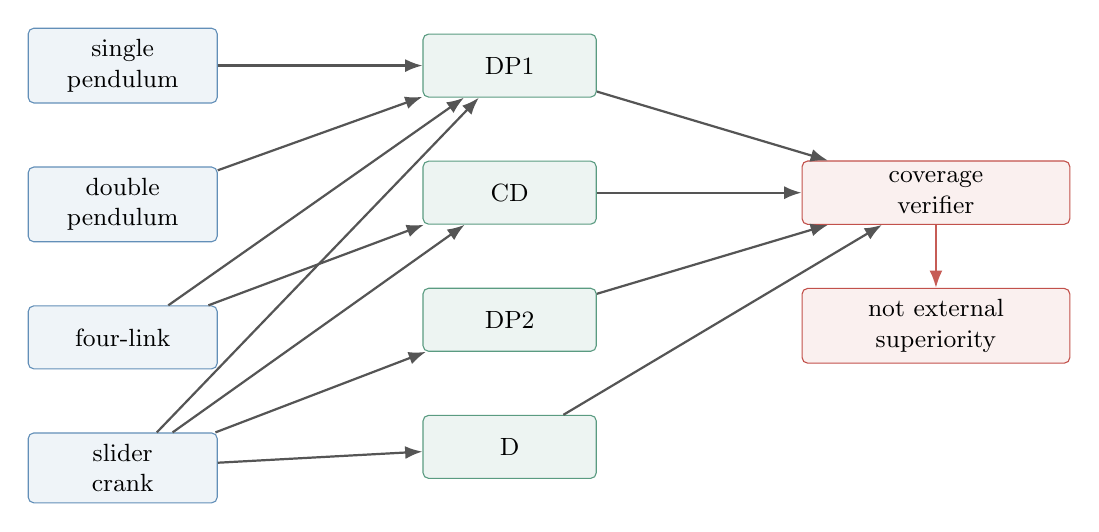
\begin{tikzpicture}[node distance=8mm and 12mm]
\node[paperbox, minimum width=24mm] (single) {single\\pendulum};
\node[paperbox, below=of single, minimum width=24mm] (double) {double\\pendulum};
\node[paperbox, below=of double, minimum width=24mm] (four) {four-link};
\node[paperbox, below=of four, minimum width=24mm] (slider) {slider\\crank};

\node[verifierbox, right=26mm of single, minimum width=22mm] (dp1) {DP1};
\node[verifierbox, below=of dp1, minimum width=22mm] (cd) {CD};
\node[verifierbox, below=of cd, minimum width=22mm] (dp2) {DP2};
\node[verifierbox, below=of dp2, minimum width=22mm] (dist) {D};

\node[boundarybox, right=26mm of cd, minimum width=34mm] (coverage) {coverage\\verifier};
\node[boundarybox, below=of coverage, minimum width=34mm] (claim) {not external\\superiority};

\draw[paperarrow] (single) -- (dp1);
\draw[paperarrow] (double) -- (dp1);
\draw[paperarrow] (four) -- (dp1);
\draw[paperarrow] (four) -- (cd);
\draw[paperarrow] (slider) -- (dp1);
\draw[paperarrow] (slider) -- (dp2);
\draw[paperarrow] (slider) -- (cd);
\draw[paperarrow] (slider) -- (dist);
\draw[paperarrow] (dp1) -- (coverage);
\draw[paperarrow] (cd) -- (coverage);
\draw[paperarrow] (dp2) -- (coverage);
\draw[paperarrow] (dist) -- (coverage);
\draw[claimarrow] (coverage) -- (claim);
\end{tikzpicture}}
\caption{The lower-pair graph bridge connects mechanism examples to constraint
families. It is a coverage and consistency verifier, not by itself an
external-superiority claim.}
\label{fig:asme}
\end{figure}

\subsection{Open caveats}

The current caveats are not secondary details; they are part of the method.
Sharp-friction coarse-regime order remains practically reduced even though
ultra refinement can recover high-order behavior at quantified cost. Sparse
structure is correct and quantified, but the dense \texttt{jacfwd} backend
remains faster in recorded wall-clock evidence. Full source-paper TFE stage
replacement remains open. External source-policy superiority remains false
because the full same-test benchmark campaign has not been run.

\begin{figure}[t]
\centering
\begin{minipage}{0.48\linewidth}
\centering

\includegraphics[width=\linewidth]{friction_smoothness_sweep.png}
\end{minipage}
\hfill
\begin{minipage}{0.48\linewidth}
\centering

\includegraphics[width=\linewidth]{sparse_speed_gap.png}
\end{minipage}
\caption{Two caveats that the agent must preserve: sharp-friction smoothness
and sparse-backend runtime. Both are useful evidence streams, but neither
supports an overbroad claim.}
\label{fig:caveats}
\end{figure}

\subsection{Claim boundary}

Figure \ref{fig:claim_boundary} summarizes the paper-facing boundary. The
accepted claim is a narrowed conditional method claim. Diagnostic evidence
remains available for future research, but not all diagnostics become claims.
Open gates include source-policy external campaigns, full TFE stage
replacement, and source-policy runner-package completeness.

\begin{figure}[t]
\centering
\resizebox{0.92\linewidth}{!}{%
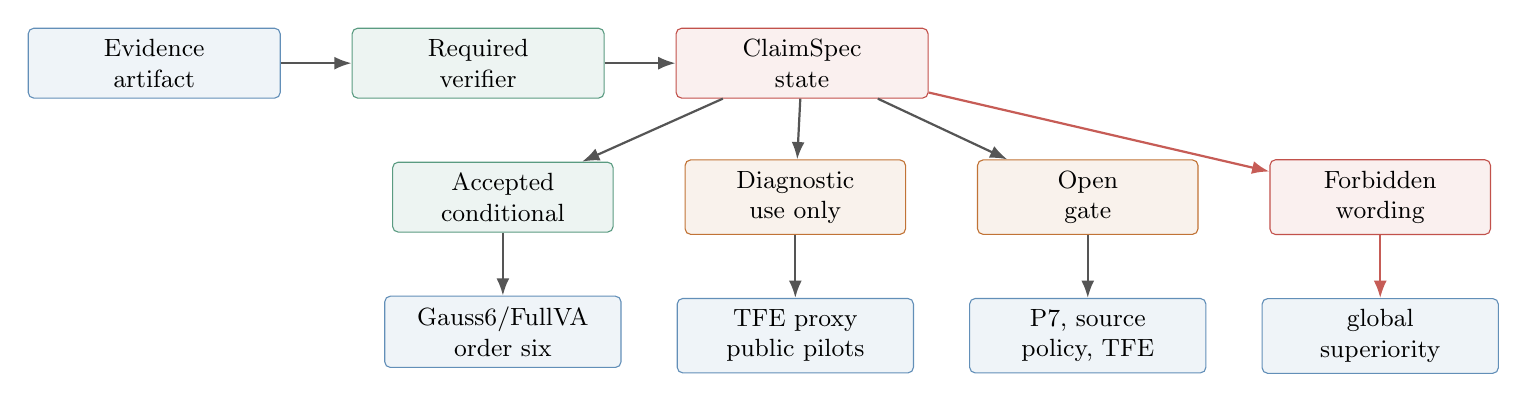
\begin{tikzpicture}[node distance=8mm and 9mm]
\node[paperbox, minimum width=32mm] (evidence) {Evidence\\artifact};
\node[verifierbox, right=of evidence, minimum width=32mm] (verifier) {Required\\verifier};
\node[boundarybox, right=of verifier, minimum width=32mm] (state) {ClaimSpec\\state};

\node[verifierbox, below=of state, xshift=-38mm, minimum width=28mm] (accepted) {Accepted\\conditional};
\node[warningbox, right=of accepted, minimum width=28mm] (diag) {Diagnostic\\use only};
\node[warningbox, right=of diag, minimum width=28mm] (open) {Open\\gate};
\node[boundarybox, right=of open, minimum width=28mm] (forbid) {Forbidden\\wording};

\node[paperbox, below=of accepted, minimum width=30mm] (methodclaim) {\method{}\\order six};
\node[paperbox, below=of diag, minimum width=30mm] (diagclaim) {TFE proxy\\public pilots};
\node[paperbox, below=of open, minimum width=30mm] (opengate) {P7, source\\policy, TFE};
\node[paperbox, below=of forbid, minimum width=30mm] (bad) {global\\superiority};

\draw[paperarrow] (evidence) -- (verifier);
\draw[paperarrow] (verifier) -- (state);
\draw[paperarrow] (state) -- (accepted);
\draw[paperarrow] (state) -- (diag);
\draw[paperarrow] (state) -- (open);
\draw[claimarrow] (state) -- (forbid);
\draw[paperarrow] (accepted) -- (methodclaim);
\draw[paperarrow] (diag) -- (diagclaim);
\draw[paperarrow] (open) -- (opengate);
\draw[claimarrow] (forbid) -- (bad);
\end{tikzpicture}}
\caption{The claim boundary is part of the agent interface. Accepted evidence,
diagnostics, and open gates are shown together so that paper prose cannot
silently exceed the artifacts.}
\label{fig:claim_boundary}
\end{figure}

\section{Discussion}

\subsection{What the agent changes}

The proposed agent changes the research workflow in three ways. First, it
turns method identity into data. A candidate is not just a code path; it is a
MethodSpec whose residual rows, endpoint map, solver policy, and theorem
conditions can be audited. Second, it makes execution policy explicit. The
agent decides whether a question needs a read-only validator, a bounded probe,
a full generator, or an external campaign before running commands. Third, it
turns paper writing into a claim-state transition rather than a summarization
task.

This does not remove the human researcher. The human still chooses the
scientific direction: whether to prioritize a stronger TFE replacement, a
better sparse backend, a closed-loop dynamic-order theorem, or an external
source-policy campaign. The agent's role is to prevent the chosen direction
from corrupting the existing evidence boundary.

\subsection{Why generic agents are insufficient}

A generic coding agent can edit scripts and run tests, but integrator research
requires a different notion of correctness. The unit of progress is not
``test passed.'' It is ``a specific claim state changed under a specific
evidence policy.'' Without this discipline, an agent is likely to make the
most common research mistakes: collapsing diagnostics into claims, comparing
against mismatched baselines, or describing a mechanically buildable package as
submission-ready.

\subsection{Limitations}

This paper is a methodology and case-study paper, not a controlled evaluation
of agent productivity across laboratories. The architecture is grounded in a
single research tree for Lie-group multibody integrators. The numerical values
reported here summarize local artifacts rather than newly executed
experiments. The current v047/v048 state is also intentionally incomplete:
source-policy external superiority is false, full TFE stage replacement is not
accepted, and full global submission readiness is not claimed. These
limitations are not hidden; they are exactly the boundaries that the agent is
designed to preserve.

\section{Conclusion}

Auto-research agents for numerical-method development should be built around
verifiers, not around unconstrained autonomy. In Lie-group multibody integrator
research, the agent must preserve method identity, choose sandbox levels,
separate theorem inputs from diagnostics, select numerical examples by failure
mode, and write claims through a state machine. The v001--v048 case study shows
why this structure is necessary: each phase of the project exposed a new
failure mode, and each failure mode required a new verifier. The current
\method{} pipeline demonstrates a bounded but useful result: a conditional
sixth-order local method claim with strong smooth evidence and four ASME
mechanism rows, while retaining explicit caveats around full TFE replacement,
external source-policy campaigns, sparse speed, and sharp-friction cost. A
good agent in this setting is therefore not the one that writes the boldest
paper. It is the one that keeps the paper aligned with the proof ledger and the
artifacts.

\section*{Data and Artifact Availability}

The manuscript draft is based on local project artifacts in the
\texttt{lie\_group\_integrator\_work} tree:
\begin{itemize}
  \item \texttt{CURRENT\_PIPELINE\_CONTRACT.md};
  \item \texttt{version\_ledger.csv};
  \item \texttt{ORDER\_PROOF\_LEDGER.md};
  \item \texttt{paper\_v047\_cylindrical\_chain/CURRENT\_STATUS\_CN.md};
  \item \texttt{paper\_v047\_cylindrical\_chain/PAPER\_NUMERICAL\_RESULT\_MATRIX.md};
  \item \texttt{paper\_v047\_cylindrical\_chain/CROSS\_PAPER\_BENCHMARK\_SPEC.md};
  \item \texttt{paper\_v047\_cylindrical\_chain/CMAME\_PROOF\_CONTRACT\_GATE.md};
  \item \texttt{paper\_v047\_cylindrical\_chain/PROOF\_CLAIM\_TRACEABILITY\_AUDIT.md};
  \item \texttt{v047\_cylindrical\_chain\_pipeline/results/summary\_v047.json};
  \item \texttt{v048\_cross\_paper\_same\_test\_benchmarks/results/summary\_v048.json}.
\end{itemize}
The numerical plots are drawn from the corresponding v047 paper figure
directory; architecture, proof, ASME-lane, and claim-boundary diagrams are
rendered as LaTeX/TikZ vector figures in this source. This draft revision also
records its local reviewer pass in
\texttt{integrator\_agent\_methodology\_review\_audit.md}.

\section*{Acknowledgments}

This draft frames a methodology for coordinating lab-scale integrator
research. It uses the Simulation-Based Engineering Laboratory's versioned
multibody integrator artifacts as the running case study.

\begin{thebibliography}{99}

\bibitem{chaturvedi2026tfe}
E. Chaturvedi, C. Sandu, and A. Sandu.
Higher-order integration of index-3 DAE with friction using time finite
elements on Lie groups.
\emph{Multibody System Dynamics}, 2026.
doi:10.1007/s11044-026-10153-w.

\bibitem{kim2017higher}
W. Kim and J. N. Reddy.
A new family of higher-order time integration algorithms for the analysis of
structural dynamics.
\emph{Journal of Applied Mechanics}, 84(7):071008, 2017.
doi:10.1115/1.4036821.

\bibitem{hairer1996solving}
E. Hairer and G. Wanner.
\emph{Solving Ordinary Differential Equations II: Stiff and
Differential-Algebraic Problems}.
Springer, Berlin, 1996.

\bibitem{gear1985automatic}
C. W. Gear, B. Leimkuhler, and G. K. Gupta.
Automatic integration of Euler--Lagrange equations with constraints.
\emph{Journal of Computational and Applied Mathematics}, 12--13:77--90, 1985.
doi:10.1016/0377-0427(85)90008-1.

\bibitem{munthe1998lie}
H. Munthe-Kaas.
Runge--Kutta methods on Lie groups.
\emph{BIT Numerical Mathematics}, 38:92--111, 1998.

\bibitem{munthe1999high}
H. Munthe-Kaas.
High order Runge--Kutta methods on manifolds.
\emph{Applied Numerical Mathematics}, 29:115--127, 1999.

\bibitem{bruls2012lie}
O. Bruls, A. Cardona, and M. Arnold.
Lie group generalized-alpha time integration of constrained flexible
multibody systems.
\emph{Mechanism and Machine Theory}, 48:121--137, 2012.
doi:10.1016/j.mechmachtheory.2011.07.017.

\bibitem{wieloch2021bdf}
V. Wieloch and M. Arnold.
BDF integrators for constrained mechanical systems on Lie groups.
\emph{Journal of Computational and Applied Mathematics}, 387:112517, 2021.
doi:10.1016/j.cam.2019.112517.

\bibitem{jay1996symplectic}
L. O. Jay.
Symplectic partitioned Runge--Kutta methods for constrained Hamiltonian
systems.
\emph{SIAM Journal on Numerical Analysis}, 33(1):368--387, 1996.
doi:10.1137/0733019.

\bibitem{marsden2001discrete}
J. E. Marsden and M. West.
Discrete mechanics and variational integrators.
\emph{Acta Numerica}, 10:357--514, 2001.
doi:10.1017/S096249290100006X.

\bibitem{leyendecker2008variational}
S. Leyendecker, J. E. Marsden, and M. Ortiz.
Variational integrators for constrained dynamical systems.
\emph{ZAMM}, 88(9):677--708, 2008.
doi:10.1002/zamm.200700173.

\bibitem{stewart1996implicit}
D. E. Stewart and J. C. Trinkle.
An implicit time-stepping scheme for rigid body dynamics with inelastic
collisions and Coulomb friction.
\emph{International Journal for Numerical Methods in Engineering},
39(15):2673--2691, 1996.
doi:10.1002/(SICI)1097-0207(19960815)39:15<2673::AID-NME972>3.0.CO;2-I.

\bibitem{anitescu1997formulating}
M. Anitescu and F. A. Potra.
Formulating dynamic multi-rigid-body contact problems with friction as
solvable linear complementarity problems.
\emph{Nonlinear Dynamics}, 14(3):231--247, 1997.
doi:10.1023/A:1008292328909.

\bibitem{tasora2011matrixfree}
A. Tasora and M. Anitescu.
A matrix-free cone complementarity approach for solving large-scale,
nonsmooth, rigid body dynamics.
\emph{Computer Methods in Applied Mechanics and Engineering}, 200:439--453,
2011.
doi:10.1016/j.cma.2010.06.030.

\bibitem{borri1988rigid}
M. Borri and S. N. Atluri.
Time-finite element method for the constrained dynamics of a rigid body.
In \emph{Computational Mechanics}. Springer, Berlin, 1988.

\bibitem{hughes1988spacetime}
T. J. R. Hughes and G. M. Hulbert.
Space-time finite element formulations for elastodynamics: formulations and
error estimates.
\emph{Computer Methods in Applied Mechanics and Engineering}, 66:339--363,
1988.

\bibitem{hulbert1992time}
G. M. Hulbert.
Time finite element methods for structural dynamics.
\emph{International Journal for Numerical Methods in Engineering}, 33:307--331,
1992.

\bibitem{jog2016robust}
C. S. Jog, M. Agrawal, and A. Nandy.
The time finite element as a robust general scheme for solving nonlinear
dynamic equations including chaotic systems.
\emph{Applied Mathematics and Computation}, 279:43--61, 2016.

\bibitem{bauchau2024time}
O. A. Bauchau.
The finite element method in time for multibody dynamics.
\emph{Journal of Computational and Nonlinear Dynamics}, 19(7):071001, 2024.
doi:10.1115/1.4063953.

\bibitem{brown2016friction}
P. Brown and J. McPhee.
A continuous velocity-based friction model for dynamics and control with
physically meaningful parameters.
\emph{Journal of Computational and Nonlinear Dynamics}, 11:054502, 2016.
doi:10.1115/1.4033658.

\bibitem{taves2020exponential}
J. Taves, A. Kissel, and D. Negrut.
On an exponential map approach for rigid body kinematics and dynamics
analysis.
Technical Report TR-2020-08, Simulation-Based Engineering Laboratory,
University of Wisconsin--Madison, 2020.

\bibitem{kissel2021dwelling}
A. Kissel, D. Negrut, and J. Taves.
Dwelling on the connection between SO(3) and rotation matrices in rigid
multibody dynamics. Part 1: Description of an index-3 DAE solution approach.
In \emph{ASME IDETC-CIE}, 2021.
doi:10.1115/DETC2021-72057.

\bibitem{kissel2022absolute}
A. Kissel, D. Negrut, and J. Taves.
Constrained multibody kinematics and dynamics in absolute coordinates: a
discussion of three approaches to representing rigid body rotation.
\emph{Journal of Computational and Nonlinear Dynamics}, 17(10):101008, 2022.
doi:10.1115/1.4055140.

\bibitem{fang2023halfimplicit}
L. Fang, A. Kissel, R. Zhang, and D. Negrut.
On the use of half-implicit numerical integration in multibody dynamics.
\emph{Journal of Computational and Nonlinear Dynamics}, 18(1):014501, 2023.
doi:10.1115/1.4056183.

\bibitem{kissel2024velocitypartitioning}
A. Kissel, L. Bakke, and D. Negrut.
Reducing the constrained multibody dynamics problem to the solution of a
system of ordinary differential equations via velocity partitioning and Lie
group integration.
\emph{Journal of Computational and Nonlinear Dynamics}, 19(7), 2024.
doi:10.1115/1.4065254.

\bibitem{localcontract2026}
J. Wang.
Current pipeline contract and v047/v048 claim-boundary artifacts.
Local project artifacts in \texttt{lie\_group\_integrator\_work}, 2026.

\end{thebibliography}

\end{document}
